%================================================
%美国大学生数学建模竞赛
%COMAP's Interdisciplinary Contest In Modeling
%================================================
%2023年2月21日 定稿
%February 21, 2023 Finalized
%================================================
%队伍成员: 郑竣哲、韩林霈、张祎
%Team Menbers: Zheng Junzhe, Han Linpei, Zhang Yi
%================================================

\documentclass[12pt]{article}
\usepackage[2303193]{easymcm}
\problem{F}
\usepackage{mathptmx}  %Times 字体
\usepackage{bm} %公式中加粗
\title{Green GDP—The Key to Sustainable Economic Development}  %标题
\begin{document} %论文开始
	\begin{abstract} %摘要
	As the concept of high-quality development continues to take root in people's hearts, how to achieve a healthier and more balanced economic development has become the top priority of many countries.
	Obviously, the old method of calculating \textit{GDP} can no longer meet today's requirements.
	In order to measure a country's economic health more realistically, we have comprehensively designed a new scheme - \textit{GGDP}, based on the essence of the production method and combined with multiple methods such as \textbf{Multiple Linear Regression} and \textbf{Weight Analysis}. 
	
	\textbf{For Question 1}, we use the \textbf{Linear Regression Method} to build a model of the relationship between a country's \textit{GGDP} and the world climate and environment.
	Taking \textit{GGDP} as a dependent variable, global carbon dioxide emissions and the proportion of global renewable energy power generation as independent variables, the conclusions of the two sets of data are more linear.
	The detailed analysis process is reflected in \textbf{Section \ref{task2}}.
	Finally, we get the result that the \textit{GDP} of a large country is negatively correlated with the global carbon dioxide emissions and positively correlated with the proportion of global renewable energy power generation.
	That’s to say, the adoption of \textit{GDP} as the main indicator will have a positive impact on the global climate and environment.
	
	
	\textbf{For Question 2}, we use Delphi method to investigate the staff at all professional levels and analyze the data for \textbf{Weight Analysis}.
	At the same time, we quantify the advantages and disadvantages of \textit{GGDP}.
	It is concluded that the advantages of \textit{GGDP} are far greater than the potential disadvantages.
	The negative impact of \textit{GGDP} on \textit{GDP} is predicted and fitted by the method of partial least squares.
	The detailed operational analysis is reflected in \textbf{Section \ref{task3}}.
	Finally, it is concluded that the negative impact of \textit{GGDP} on \textit{GDP} growth rate is relatively small, and the advantages of \textit{GGDP} are far greater than disadvantages.
	
	
	\textbf{For Question 3}, we selected representative indicators, and assigned appropriate weights to each indicator using \textbf{Entropy Weighting Method}(EWM).
	Based on these weights, we used \textbf{TOPSIS} method to obtain the comprehensive evaluation index as the approximate value of \textit{GGDP}, and obtained the \textit{GGDP} data in the time dimension.
	At the same time, we obtain data from the time dimension of \textit{GDP}.
	After analyzing and comparing these two data, we find that the decay rate of \textit{GGDP} data growth is significantly greater than that of \textit{GDP} data growth rate, which shows that \textit{GDP} cannot represent the loss of natural resources.
	Finally, it is concluded that after the adoption of \textit{GDP} accounting method, China will have the support of data in formulating its sustainable development strategy, which is very beneficial to the conservation of natural resources.
	
	The \textbf{GM(1,1)} is used for short-term prediction of the above data, and the results show that the growth decay rate of \textit{GGDP} is significantly lower than \textit{GDP} under the calculation method of \textit{GDP}.
	This shows that the introduction of the \textit{GGDP} accounting method can digitize the economic growth rate and thus improve the economic performance.
	This is a great support for the sustainability and rationality of economic development.
	
	Finally, we carried out \textbf{Sensitivity Analysis} and \textbf{Optimization Improvement} on the relevant models, and found that the \textbf{Binary Linear Regression} error value is extremely low, which fully demonstrates the reliability and applicability of the model.
	And the results also have great application value.
		
		% 美赛论文中无需注明关键字。若您一定要使用,
		% 请将以下两行的注释号 '%' 去除,以使其生效
	\vspace{5pt}
	\textbf{Keywords}: Green GDP(\textit{GGDP}), EWM, AHP, TOPSIS, Grey System, Multiple Linear Regression, ARIMA, RANSAC, \LaTeX.
		
	\end{abstract}
	\maketitle  % 生成 Summary Sheet
	\tableofcontents  % 生成目录	
	% 正文开始
	\section{Non-technical Reporting} %非技术性报告
	
	According to the models and cases we have built, and based on national conditions, it is obvious that shifting to \textit{GGDP} plays a more important role in the country's economic health.
	There are some irreparable drawbacks of the old \textit{GDP} model, such as the failure to reflect the impact of economic development on the natural environment, which is an indicator designed to reflect the relationship between economic development and environmental sustainability.
	It includes environmental considerations, such as clean energy, ecosystem services and pollution control and so on.
	The emergence of \textit{GGDP} highlights the coordination between environmental sustainability and economic development.
	
	In addition, \textit{GGDP} has some other advantages over \textit{GDP}.
	From the perspective of environmental sustainability, \textit{GGDP} can better reflect the impact of economic development on the environment and provide more accurate reference and guidance for environmental governance.
	From the perspective of the comprehensiveness of economic indicators, \textit{GGDP} takes into account economic, social and environmental factors, can provide a more comprehensive assessment and comparison, and effectively reduces the defect that traditional \textit{GDP} ignores non-economic factors.
	In addition, in the long run, \textit{GGDP} can better reflect the long-term impact of economic development, especially on the environment, which helps to formulate long-term sustainable development strategies and policies.
	
	Although \textit{GGDP} has many unparalleled advantages, the promotion of \textit{GGDP} requires governments and society due to the relatively short time to put forward concepts, data collection and calculation, accurate definitions and specific indicator systems, and how to trade-offs between the economy, society and the environment.
	Therefore, the promotion of \textit{GGDP} requires governments and society.
	The broad support and participation of the community requires greater investment and dedication.
	
	At the same time, due to differences in values of environmental and social benefits, some people may focus more on economic growth, while others may pay more attention to environmental sustainability, which may affect the assessment and application of \textit{GGDP}.
	And \textit{GGDP} is a relatively new concept, and there is a lack of unified international standards, which may limit its global application.
	
	In the initial stage, \textit{GGDP} is a perfect choice as an auxiliary index of \textit{GDP}.
	\textit{GGDP} is an indicator with great potential to more comprehensively assess the relationship between economic development and environmental sustainability.
	Even if many difficulties and challenges still need to be overcome to truly play its role, \textit{GGDP} deserves government input to solve these difficulties in order to facilitate the full release of the potential of \textit{GGDP}.
	
	\newpage
	
	\section{Introduction} %介绍
	\subsection{Problem Background} %问题背景
	Over time, in pursuit of social-economic development, countries use \textit{GDP} as an indicator of a country's economic health. Usually, a country's \textit{GDP} can determine the country's import and export trade and the right to apply for state loans.
	Therefore, while focusing on \textit{GDP} development, countries have contributed to today's production, but it has a great negative impact on the environment.
	For example, there are large tropical rainforests in northern Brazil. Because their country has a large population and weak productivity in the secondary industry, some people have cut down the northern Amazon in order to increase \textit{GDP}.
	Trees in tropical rainforests produce a large amount of wooden furniture.
	However, the country's behavior will lead to the reduction of global forest area, the reduction of biodiversity and the disorder of the global carbon balance.
	In order to reduce investment in environmental pollution control, the same coastal country dumps nuclear wastewater directly into the ocean without considering the pollution damage to the marine ecological environment.
	Failure to impose penalties may have an irreversible impact on the global marine ecological environment.
	
	Therefore, we believe that \textit{GDP} is not a good measure of healthy national economic development.
	If nations change the ways they evaluate and compare their economies, national governments may change their behaviors, promoting policies and projects that are better for the environmental health of the planet.
	So we consider whether \textit{GGDP} can be used as this indicator.
	
	Three major problems are discussed in this paper, which are:
	
	\begin{itemize}
		\item Ensuring that a country adopts a \textit{GGDP} will have a positive impact on the global climate environment.
		\item Ensuring that \textit{GGDP} replaces \textit{GDP} as an indicator that mainly measures the healthy development of the country's economy outweighs the disadvantages.
		\item We select China and inquire about detailed data for in-depth analysis and research to ensure that the implementation of \textit{GGDP} will enable the government to implement special policies on the use of natural resources and investment in environmental pollution control.
		This policy is also an economic policy for sustainable development for future generations.
	\end{itemize}
	
	\subsection{Literature Review} % 文献回顾
	Through the inquiry of the literature, we decided to use the production method as a way to calculate \textit{GGDP} in our paper.
	Some literatures use the \textbf{EWM} to evaluate the impact of \textit{GGDP}.
	We believe that various data can be weighted and analyzed in combination with a variety of evaluation methods to make the results more accurate and realistic.
	
	\newpage
	
	\subsection{Our Work} %我们干了什么 一张思维导图
	
	\begin{figure}[!htbp]
		\centering
		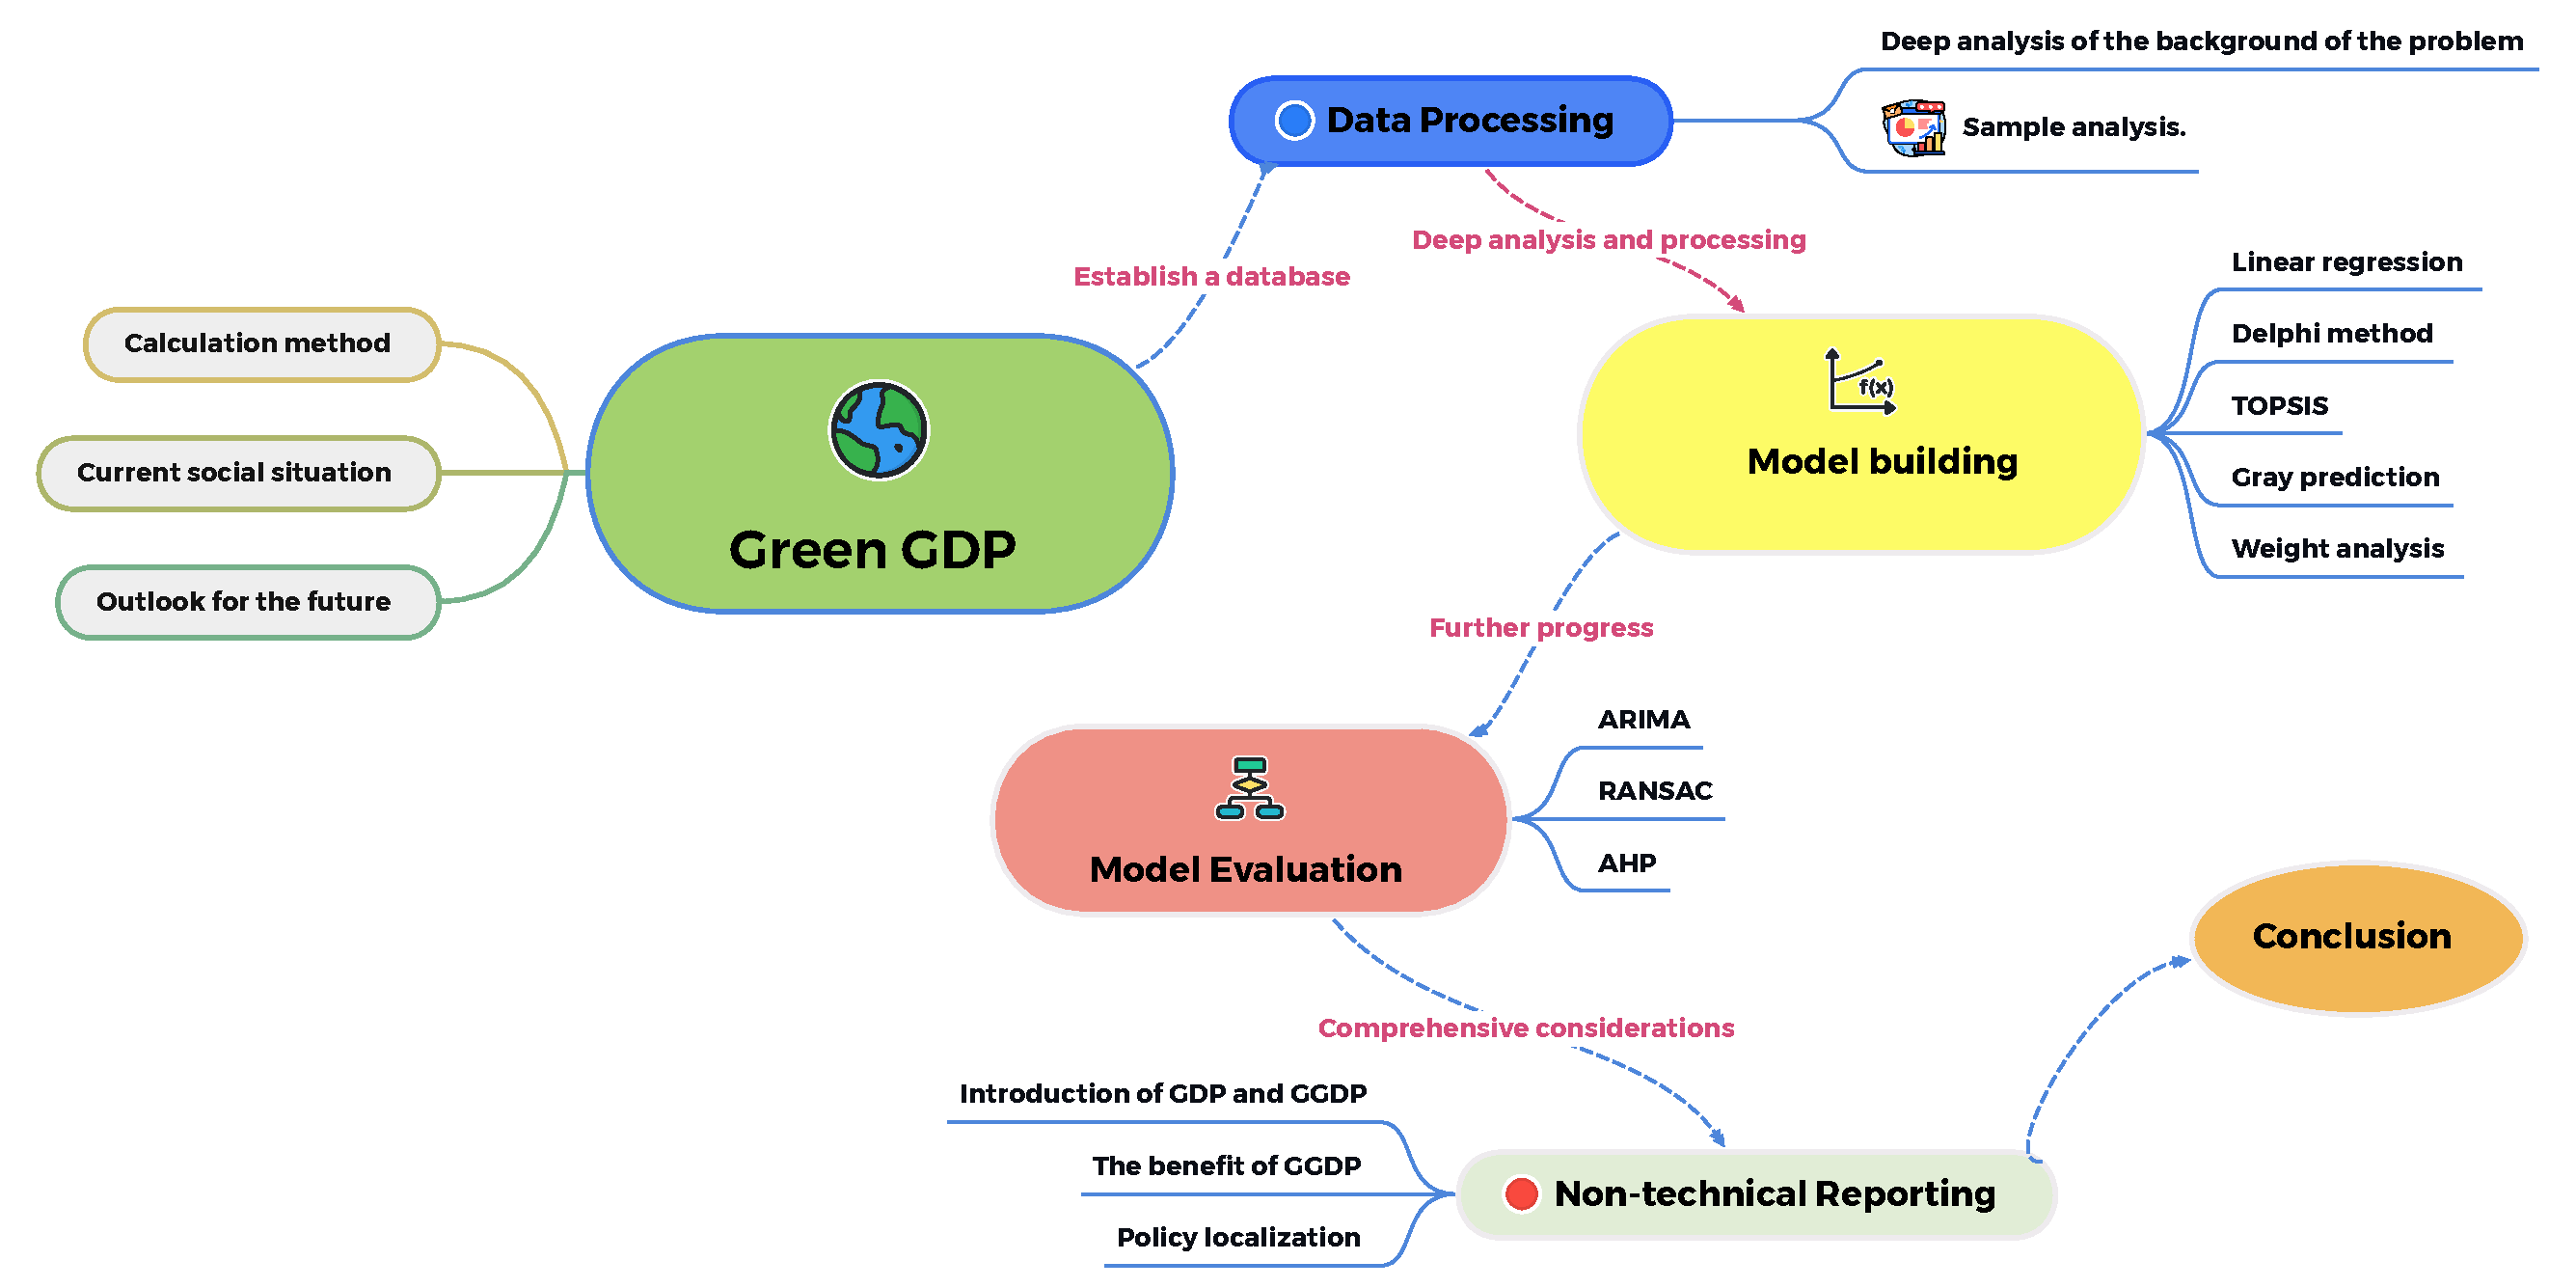
\includegraphics[width=\textwidth]{GreenGDP.pdf}
		\caption{Mind Map}\label{fig:mindmap}
	\end{figure}

		
	\section{Data Processing} %数据处理
	\subsection{Establishment of Complete Datasets} %建立完整的数据库 
	
	In order to establish a more authoritative, accurate and perfect database, after determining the topic, we spent several hours in data search to collect the two sets of official data from various countries with a ten-year time span from 2011 to 2020 and from 2012 to 2021, and compare the data through the establishment of models, and it is convenient to predict the climate and environment and analyze China's \textit{GGDP} and its impact on the ecological environment in the later stage.
	
	Our data are collected from official websites such as the World Bank (IBRD·IDA), the U.S. Energy Information Administration (EIA), CNKI Foreign Journal, the National Bureau of Statistics, the Chinese Government Network, and the Ministry of Ecology and Environment of China.
	\subsection{A Sample of Data Processing} %一个数据处理的样式
	In the process of collecting data, we will find that some data are lost. For example, the data on China's total wastewater discharge are missing from 2016 to 2021, and the National Bureau of Statistics has not disclosed its data, so we use its sub-data for the comprehensive operation of mean interpolation and regression interpolation. 

	
	\begin{itemize}
		\item \textbf{Mean interpolation method}
		
		Because its sub-data also has missing values, but the number of missing values is small and does not fluctuate much, we use the mean interpolation method to fill the loss of sub-data.
		
		\begin{table}[!htbp]
			\begin{center}
				\caption{Mercury-containing Wastewater Emissions}
				\label{}
				\begin{tabular}{ccccccccccc}
					\toprule
					\multicolumn{1}{m{2cm}}{\centering \textbf{Year}}
					& \multicolumn{1}{m{1cm}}{\centering \small 2012}
					& \multicolumn{1}{m{1cm}}{\centering \small 2013}
					& \multicolumn{1}{m{1cm}}{\centering \small 2014}
					& \multicolumn{1}{m{1cm}}{\centering \small 2015}
					& \multicolumn{1}{m{1cm}}{\centering \small 2016}
					& \multicolumn{1}{m{1cm}}{\centering \small 2017}
					& \multicolumn{1}{m{1cm}}{\centering \small 2018}
					& \multicolumn{1}{m{1cm}}{\centering \small 2019}
					& \multicolumn{1}{m{1cm}}{\centering \small 2020}
					& \multicolumn{1}{m{1cm}}{\centering \small 2021}\\
					\midrule
					\small \textbf{Hg}(kg) & 1223 & 917 & 746 & 1080 & 915.5 & 960.4 & 950.6 & 995.5 & 1129 & 638\\
					\bottomrule
				\end{tabular}
			\end{center}
		\end{table}
	
		\item \textbf{Regression interpolation method}
		
		Because the data missing value of the total wastewater discharge is too large, it is impossible to directly fill it with the mean interpolation method, but the missing value of sub-data is less.
		We found that the sub-data given by the Bureau of Statistics is not the complete set of total data, so we set $Y$ as the hidden data, $T$ as the total data, and the sum of each sub-data as $S$.
		We use $Y=T-S$ to get four sets of hidden data from 2012 to 2015, and then use the regression interpolation method to regress the hidden data into a function curve pair.
		The lost hidden data is predicted, and then the predicted $\hat{Y}$ is summated with the known sub-data to obtain more accurate data on the total wastewater discharge.
	\end{itemize}

	\section{Task 1} %任务一
	\subsection*{Linear Regression Model} %线性回归模型
	With the development of the world economy and society, more and more countries realize that simple \textit{GDP} cannot fully represent the country's economic situation.
	As an important part of the earth, the natural ecological environment is also an important asset owned by the country, so we chose the production method to calculate \textit{GGDP} as a more comprehensive indicator of a country's economic health.
	In order to ensure that the calculated \textit{GGDP} is really related to the climate and environment, we consulted various data from the United States and China for analysis and comparison.
	\begin{table}[!htbp]
		\begin{center}
			\caption{Generate Electricity and $CO_{2}$}
			\label{}
			\begin{tabular}{cccccc}
				\toprule
				\multicolumn{1}{m{1cm}}{\centering \textbf{Year}}
				&\multicolumn{1}{m{4cm}}{\centering \textbf{\textit{GDP}}(Trillion dollars)}
				& \multicolumn{1}{m{2cm}}{\centering \textbf{\textit{GGDP}}}
				& \multicolumn{1}{m{2.5cm}}{\centering \textbf{\textit{GGDP/GDP}}}
				& \multicolumn{1}{m{2cm}}{\centering \textbf{GREG}(\%)}
				& \multicolumn{1}{m{2cm}}{\centering \bm{$CO_{2}$}{$(kt)$}}\\
				\midrule
				2011 & 15.6 & 12.23 & 0.783974359 & 4.1 & 32,021,108.0\\
				2012 & 16.25 & 12.51 & 0.769846154 & 4.7 & 32,460,317.0\\
				2013 & 16.84 & 13.04 & 0.774346793 & 5.4 & 33,119,383.0\\
				2014 & 17.55 & 13.82 & 0.787464387 & 6 & 33,198,730.0\\
				2015 & 18.21 & 14.81 & 0.813289401 & 6.8 & 32,995,536.0\\
				2016 & 18.7 & 15.8 & 0.844919786 & 7.5 & 33,018,556.0\\
				2017 & 19.48 & 16.92 & 0.868583162 & 7 & 33,514,538.0\\
				2018 & 20.53 & 17.96 & 0.87481734 & 8 & 34,289,351.0\\
				2019 & 21.38 & 19.02 & 0.889616464 & 8.8 & 34,344,006.0\\
				2020 & 21.06 & 20.1 & 0.954415954 & 9.1 & 32,284,000.0\\
				\bottomrule
			\end{tabular}
		\end{center}
	\end{table}
	
	
	\subsection{Least Squares Approximation} %最小二乘法
	In the process of analysis, we found that the value of \textit{GGDP} in the United States and global greenhouse gas emissions represented by CO2 are negatively correlated with the functional curve of U.S.\textit{GDP}; the value of \textit{GGDP} in the United States is positively correlated with the proportion of global renewable energy generation and \textit{GDP} is negatively correlated with it, so we use the least squares approximation to fit the linear regression model.
	
	In our regression analysis, a linear relationship composed of two independent variables and a dependent variable can get the following regression model:
	
	\begin{equation}\label{}
		y=\beta _{0}+\beta _{1}x_{1}+\beta_{2}x_{2}+...\beta_{k}x_{x}+\varepsilon
	\end{equation}
	
	First of all, the data is organized in the form of a matrix, and the solution of $\beta$ is calculated by the least square method:
	
	\begin{equation}\label{}
		\hat{\beta } =(\left [ x_{ij} \right ]^{\top } \left [ x_{ij} \right ] )^{-1}\left [ x_{ij} \right ] ^{\top}\left [ y_{ij} \right ]
	\end{equation}
	
	Then use $\sigma$ to calculate the value of slope $b$:
	
	\begin{equation}\label{}
		u(b)=\frac{\sigma }{\sqrt{\sum (x-\bar{x} )^{2}} }
	\end{equation}
	
	Finally, the binary linear regression equation can be obtained. 
	
	\subsection{Fitting Binary Linear Regression Equation} %拟合二元线性回归方程
	The constructed functional model.
	
	\begin{equation}\label{}
		\hat{y}_{CO_{2}} = 18088441.136 + 1749908.831x_{GDP}-1116586.424x_{GGDP}
	\end{equation}
	\begin{equation}\label{}
		\hat{y}_{energy}  =-7 .343 + 0.1x_{GGDP}+0.675x_{GDP}
	\end{equation}
	Through this model, it can be concluded that greenhouse gas emissions represented by carbon dioxide are negatively correlated with \textit{GGDP}, and the proportion of global renewable energy generation is positively correlated with \textit{GGDP}.
	Therefore, it can be concluded that with the use of \textit{GGDP} instead of \textit{GDP}, it explains the emission of greenhouse gases with the increase of \textit{GGDP}.
	Similarly, water pollution and solid pollution will also show a corresponding trend of reduction.
	
	\subsection{Regression Formula Verification} %回归公式验证
	Through the binary regression equation curves fitted by the least squares approximation, the significance is 0.0001\% and 0.003\% respectively.
	Therefore, the curves proposed in this model are very accurate, and future values can be predicted more accurately.
	From the above, it can be seen that if a country adopts \textit{GGDP} as the main indicator of a country's economic health, as the ratio of \textit{GGDP} and \textit{GGDP}/\textit{GDP} rises, the country's climate environment will improve, which can play a positive role in the global climate environment.

	\subsection{Conclusion of The Problem} %问题的结论	
	The impact of the United States' application of \textit{GGDP} as the main measure of national economic health development indicators on global carbon dioxide emissions and the proportion of global renewable energy power generation can be seen, the results of its improvement of the global climate environment can be drawn.
	Therefore, we believe that \textit{GGDP} can be used as the main indicator, taking into account \textit{GDP} and some other social factors to analyze and evaluate national development.
		
	\section{Task 2}\label{task2} %任务二	
	\subsection*{Delphi Method \& Weight Analysis \& Linear Regression Method} %德尔菲法、权重分析法、线性回归法
	There must be some resistance in deciding to replace \textit{GDP} with \textit{GGDP} as an important indicator of a country's main measure of healthy economic development. 
	Because \textit{GGDP} also has potential disadvantages corresponding to it, such as the difficulty of data collection and large calculation of \textit{GGDP}, different definitions and calculation weights by countries, and different values of individuals or governments.
	
	In order to ensure that the advantages of using \textit{GGDP} far outweigh the disadvantages, we intend to use Delphia investigates workers at all levels of society, including college students, government employees, hospital workers, state-owned enterprises and private enterprise workers.
	Our questionnaire covers six directions, three of which are the advantages of \textit{GGDP} and the other three are the potential disadvantages of \textit{GGDP}, so that the respondents can more fully express their personal opinions.
	
	In order to make the results of Delphi method more accurate, the audience we proposed the questionnaire are all from environment-related or economic-related majors, such as undergraduates in economics, graduate students of environmental protection, director of the Planning Office of the Environmental Protection Agency, and so on.
	The process took about a day to complete.
	
	Therefore, the proportion selected according to the three questionnaire options is only a table, forming the following table.
	
	
	\begin{table}[!htbp]
		\begin{center}
			\caption{Delphi Method}
			\label{}
			\begin{tabular}{ccccccc}
				\toprule
				\multicolumn{1}{m{3cm}}{\centering \textbf{Year}}
				& \multicolumn{1}{m{1.5cm}}{\centering 2012}
				& \multicolumn{1}{m{1.5cm}}{\centering 2013}
				& \multicolumn{1}{m{1.5cm}}{\centering 2014}
				& \multicolumn{1}{m{1.5cm}}{\centering 2015}
				& \multicolumn{1}{m{1.5cm}}{\centering 2016}
				& \multicolumn{1}{m{1.5cm}}{\centering 2017}\\
				\midrule
				\textbf{First} & 0.86 & 0.89 & 0.93 & 0.03 & 0.06 & 0.12 \\
				\textbf{Second} & 0.9 & 0.83 & 0.91 & 0.05 & 0.07 & 0.07 \\
				\textbf{Third} & 0.88 & 0.9 & 0.95 & 0.04 & 0.06 & 0.11 \\
				\bottomrule
			\end{tabular}
		\end{center}
	\end{table}
	
	\newpage
	
	\subsection{Weight Analysis} %权重分析
	By weighting the data of this table, it can be concluded that people at the social level are more aware of the advantages of GGDP, and their potential disadvantages are relatively small.
	From the statistical and data analysis of Delphi, it can be concluded that from the perspective of staff at all levels of society, the advantages of replacing GDP with GGDP are far greater than their potential disadvantages. 
	
	We use the formula: $\wp =\frac{m_{i}}{\sum_{i=1}^{n} m_{i}} $ to calculate the proportion of data collected by Delphi.
	
	However, the Delphi method cannot ensure the objectivity of the results.
	In order to ensure objectivity, we have analyzed the relationship between GGDP and GGDP and GGDP/GDP in the United States in the past decade, and found that there is also a potential functional relationship between the two pairs of data.
	
	\subsection{Linear Regression} %线性回归
	With 10 years of data, in order to analyze the relationship between \textit{GGDP} and the relationship between \textit{GGDP} and the ratio of \textit{GGDP} to \textit{GGDP}/\textit{GDP}, we decided to use the least squares approximation method to fit the linear regression equation again, and finally got the formulae:
	
	\begin{equation}\label{eq:GDP}
		\hat{y}_{GDP} =7.405 + 0.714x_{GGDP}
	\end{equation}
	\begin{equation}\label{GGDP/GDP}
		\hat{y}_{GGDP/GDP} =0.505 + 0.021x_{GGDP}
	\end{equation}
	
	Through the fitting unary linear regression equation, it can be concluded that with the growth of \textit{GGDP}, \textit{GDP} and \textit{GGDP}/\textit{GDP} will increase, both with the development of \textit{GGDP}, to the national economy. The environment will have a positive impact.
	
	\begin{figure}[htbp]
		\centering
		\begin{subfigure}[b]{.4\textwidth}
			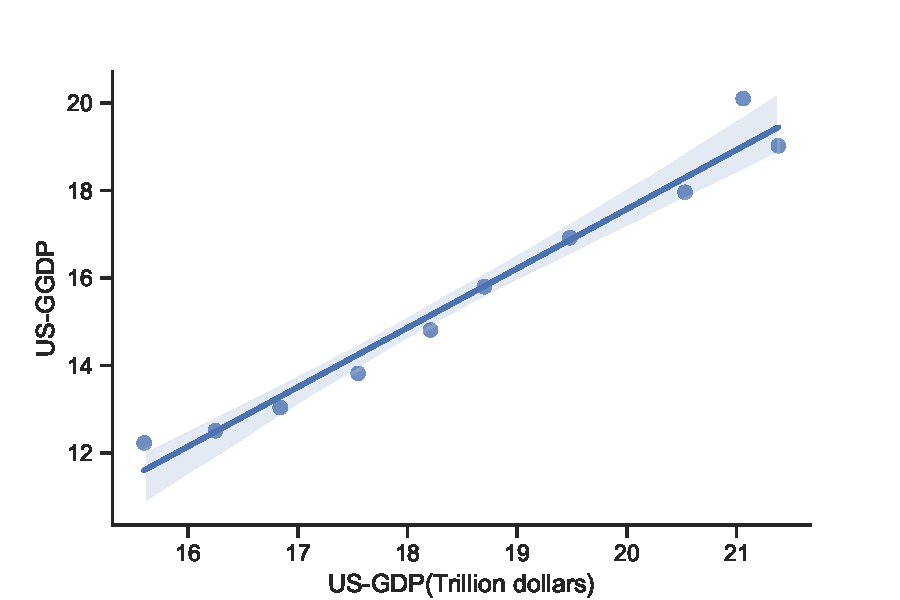
\includegraphics[width=\textwidth]{./US-GGDP-GDP/US-GGDP-GDP.pdf}
			\caption{$GGDP$-$GDP$}\label{}
		\end{subfigure}
		\begin{subfigure}[b]{.4\textwidth}
			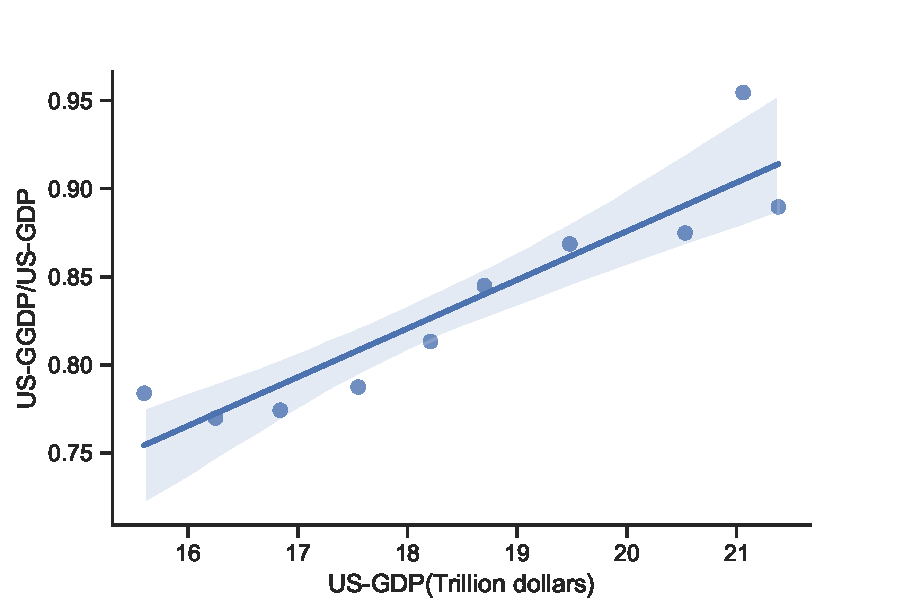
\includegraphics[width=\textwidth]{./US-GGDP-GDP/US-GGDP-GDPlv.pdf}
			\caption{$GGDP / GDP$-$GDP$}\label{}
		\end{subfigure}
		\caption{Linear equation of regression}\label{}
	\end{figure}
	
	\subsection{Significance Test} %显著性检验
	Through the significance test of linear regression equations, the significance coefficients of the two fitting linear regression equations are 0.0001\%, which basically meets the prediction requirements.
	
	\subsection{Conclusion of The Problem} %问题的结论
	The above model proves that the advantages of using \textit{GGDP} instead of \textit{GDP} as the main measure of a country's healthy economic development far outweigh the disadvantage, and the global economic and climatic environment will have an ideal trend by further increasing \textit{GGDP} in the future.
	
	\section{Task 3}\label{task3} %任务三
	\subsection{Data Preparation} %数据准备
	\subsubsection{Target selection}\label{IndexSelection} %指标选择
	\textit{GGDP} is a supplement to and perfect \textit{GDP}.
	The accounting method of introducing resource and environmental loss factors into the \textbf{SNA} can better reflect the sustainable development of a country's national economy, people and environmental problems than \textit{GDP}.
	The increasing traditional \textit{GDP} is based on the overuse of environmental resources and damage to public health, and the traditional \textit{GDP} accounting method cannot reflect these losses.
	With the development of the times, the concept of \textit{GGDP} is becoming more and more widely recognized by the international community.
	But so far, there has been no recognized and feasible \textit{GGDP} accounting model in the world, and no country has publicly released the results of \textit{GGDP}.
	The concept of \textit{GGDP} remains on paper.
	
	According to the accepted meaning of \textit{GGDP}, we take China as an example to choose the following indicators from the data released by National Bureau of Statistics of China\cite{6}.
	
	
	\begin{itemize}
		\item \textbf{National GDP(NGDP)}
		
		\textit{GGDP} is based on \textit{GDP}, so it needs to be introduced.
		
		\item \textbf{Nature reserve area(NRA) }
		
		Nature reserves can reflect a country's environmental protection.
		The larger the area of the nature reserve, the more attention the country attaches to environmental protection.
		
		\item \textbf{Urban green space(UGSA)}
		
		Urban green spaces have three functions: ecological, psychological and physical functions, which can purify air, water and soil, prevent soil erosion, improve urban microclimate, and reduce noise in cities.
		It is of great benefit to the living environment of residents.
		And green plants can stimulate people's physiological vitality and make people happy physically and mentally.
		
		\item \textbf{Forest land area(FLA)}
		
		Forest ecosystems have complex energy and material information flow, which have the functions of windproof and sand fixation, water and soil conservation, water conservation, climate regulation, and flood mitigation.
		The more forest land is used, the more attention the country attaches to forest resources.
		
		\item \textbf{Investment in industrial pollution control (IPCI)}
		
		Investment in industrial pollution control reflects a country's attitude towards pollution control.
		The higher the investment in industrial pollution control, the stronger the country's pollution control.
		
		\item \textbf{Number of harmless treatment plants(NGIDP) }
		
		Domestic waste harmless treatment factories refer to various domestic waste treatment facilities designed, constructed, operated, maintained and managed in accordance with relevant technical, environmental and hygienic standards and norms.
		It can reflect the country's garbage disposal efforts.
		The more harmless treatment plants there are, the higher the processing strength.
		
		\item \textbf{Harmless disposal rate of domestic waste(HDRDW) }
		
		The harmless disposal rate of domestic waste can reflect the country's technical level of handling domestic waste.
		The higher the harmless disposal rate of domestic waste, the higher the technical level.
		
		\item \textbf{Solid waste utilization rate(SWUR)}
		
		Solid waste is one of the sources of environmental pollution.
		It must occupy a large amount of land and cause serious pollution to soil water sources.
		Solid waste utilization can reflect the degree of the country's solution to the solid waste problem, and thus the importance the country attaches to environmental pollution.
		
		\item \textbf{Industrial capacity utilization rate(ICUR) }
		
		The utilization rate of industrial capacity can reflect the country's industrial level and the natural resources consumed in the process of industrial production.
		The higher the utilization rate of industrial production capacity, the lower the loss of natural resources.
		
		\item \textbf{Total water consumption for industry and agriculture(TWCIA) }
		
		The total amount of water used in industry and agriculture is the use of water resources in the development process.
		We can see the consumption of water resources by the country's economic development through the total amount of industrial and agricultural water.
		
		\item \textbf{Total wastewater discharge(TWD)}
		
		Wastewater is a water resource that cannot be reused by human beings through treatment, which can reflect the loss of the country's environmental resources.
		
		\item \textbf{Heavy metal emissions from wastewater(HMEW) }
		
		Heavy metals are significantly biotoxic.
		Because it is difficult to biodegrade, it can enrich thousands of times with the food chain and finally enter the human body, causing chronic poisoning.
		
		\item \textbf{Total emissions from exhaust(TEE)}
		
		Exhaust gas is a toxic and harmful gas emitted into the atmosphere by human beings in production and life.
		Exhaust gas is seriously polluted to the air.
		The more emissions are, the more serious the damage to the environment in the country.
		
		\item \textbf{Sulfur dioxide emissions(SDE)}
		
		In the atmosphere, sulfur dioxide will oxidize into sulfuric acid fog or sulfate aerosol, which is an important precursor to environmental acidification.
		Moreover, it has a synergy with smoke and dust in the atmosphere, which is harmful to human health.
		Smoke events such as the London Smoke Incident, the Mas Valley Incident and Donora are all hazards caused by this synergy.
		The damage to public health can be estimated through sulfur dioxide emissions.
		
		\item \textbf{Nitrogen oxide emissions(NOE)}
		
		Nitrogen oxide emissions are related to the use of fossil fuels.
		
		\begin{itemize}
			\item Enter the depths of the human lungs through breathing, causing bronchitis or emphysema.
			\item It can react photochemically with other pollutants in the atmosphere to form photochemical smoke.
			\item $N_{2}O$--The transformation of oxidation into nitric acid in the atmosphere is one of the causes of acid rain.
			\item $N_{2}O$ can destroy the ozone layer and increase the amount of ultraviolet radiation.
		\end{itemize}
	\end{itemize}
	
	\subsubsection{Data standardization} %数据标准化
	According to \ref{IndexSelection} for the identified indicators, we integrate by building a decision matrix X, with a total of n samples and m reviews.
	
	\begin{equation}\label{mat:decision}
		X=
		\begin{bmatrix}
			x_{11} & \cdots  & x_{1m}\\
			\vdots  & \ddots & \vdots \\
			x_{n1} & \cdots & x_{nm}
		\end{bmatrix}
	\end{equation}

	where
	
	\qquad $x_{ij}$ represents the value of the $j$ indicator of the $i$ sample.($i=1,2,3,\cdots,n;j=1,2,3,\cdots,m$)
	
	As there are both positive indicators and negative indicators, and they need to be consistent in the same dimension, positive indicators and negative indicators are treated separately.
	
	For positive indicators:
	
	\begin{equation}\label{eq:forward}
		x_{ij}^{'}= \frac{x_{ij}-\min(x_{1j},x_{2j},\cdots,x_{nj})}{\max(x_{1j},x_{2j},\cdots,x_{nj}) - \min(x_{1j},x_{2j},\cdots,x_{nj})}
	\end{equation}
	
	For negative indicators:
	
	\begin{equation}\label{eq:backward}
		x_{ij}^{'}= \frac{\max(x_{1j},x_{2j},\cdots,x_{nj})-x_{ij}}{\max(x_{1j},x_{2j},\cdots,x_{nj}) - \min(x_{1j},x_{2j},\cdots,x_{nj})}
	\end{equation}
	
	The post-processing decision matrix is$Y$
	\begin{equation}\label{mat:normalize}
		Y=
		\begin{bmatrix}
			y_{11} & \cdots  & y_{1m}\\
			\vdots  & \ddots & \vdots \\
			y_{n1} & \cdots & y_{nm}
		\end{bmatrix}
	\end{equation}
	

	
	\subsection{Models Building} %模型建立
	\subsubsection{EWM}\label{getweight}
	\textit{GGDP} is a new and multi-factoric complex index.
	Single factors cannot determine the whole evaluation system, so they should be given a certain weight according to the size of each factor.
	
	There are many ways to determine weights, such as \textbf{AHP}, \textbf{EWM}, etc.
	Among them, the hierarchical analysis method relies on the opinions of decision makers when decomposing decision-making problems, and the results are more subjective.
	This paper introduces the concept of entropy in information theory into weight determination, and uses the relational matrix based on multiple evaluation indicators to calculate the weight value, so as to avoid the subjective impact of each factor on the decision maker, and it is possible to evaluate each factor more objectively and get the weight.
	\begin{enumerate}
		\item \textbf{Information entropy}
		
		Calculate the information entropy value of the $j$ indicator according to the definition of information entropy in information theory.
		\begin{equation}\label{eq:comentropy}
			e_{j}=-\frac{1}{\ln n}  {\sum_{i = 1}^{n} y_{ij} (\ln y_{ij})}, \quad j=1,2,3,\cdots,m
		\end{equation}
		
		\item \textbf{Information utility value}
		Calculate the information utility value of item $j$ indicator
		\begin{equation}\label{eq:utility_value}
			d_{j}=1-e_{j}, \quad j=1,2,3,\cdots,m
		\end{equation}
		
		\item \textbf{Weight coefficient}
		
		Calculate the weight of the $j$ indicator
		\begin{equation}\label{eq:weight}
			w_{j}=\frac{1-e_{j}}{n-\sum_{j=1}^{m} e_{j}}, \quad j=1,2,3,\cdots,m
		\end{equation}
		where
		
		\qquad Weight coefficient$w_{j}$satisfy$\sum_{j=1}^{m} w_{j} = 1$
	\end{enumerate}
	The calculation results are shown in the figure \ref{fig:rose} below.
	
	\begin{figure}[!htbp]
		\centering
		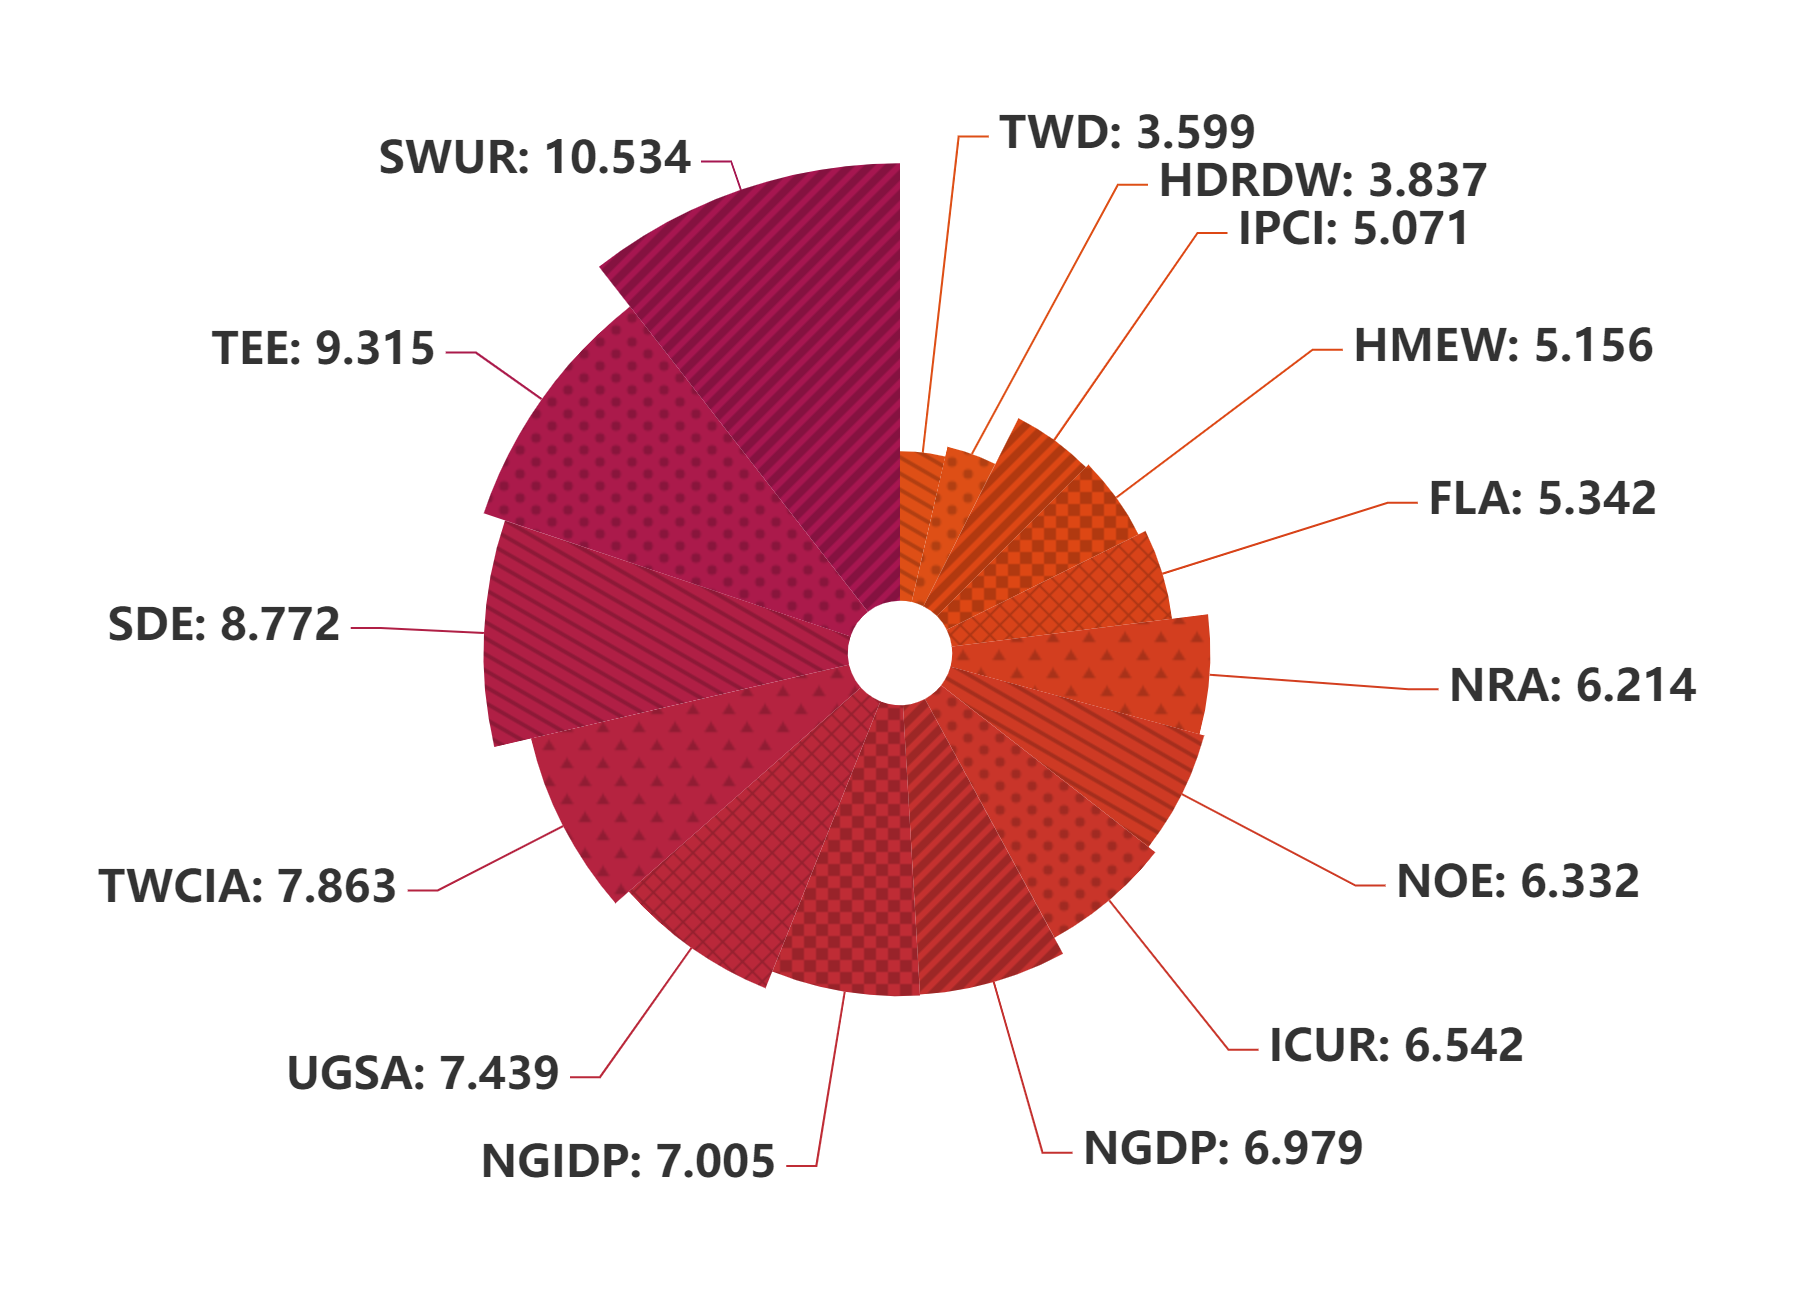
\includegraphics[width=0.6\textwidth]{ChineseDataWeightRose.png}
		\caption{Chinese Target Weight}\label{fig:rose}
	\end{figure}
	
	\subsubsection{TOPSIS}
	
	Technique for Order Preference by Similarity to an Ideal Solution(TOPSIS) is a common analytical method in multi-objective decision-making methods.
	Based on the set of options, this method treats the optimal and worst values of the calculated indicator data as a positive ideal scheme and a negative ideal scheme respectively, and calculates the distance between each scheme and the positive and negative ideal point, compares the distance between the two aspects, and finally selects the scheme closest to the positive ideal point and the most principled negative ideal point as the most excellent plan.
	
	The matrix $Y$ \eqref{mat:normalize} obtained from the weight data calculated according to \ref{getweight} Figure \ref{fig:rose} is evaluated in \textbf{TOPSIS} and ranked \textit{GGDP} by year.
	
	\begin{description}
		\item[Step1:] \textbf{Standardize}
		
		Build a standardized matrix:$Z$
		\begin{equation}\label{eq:normalization}
			z_{ij} = \frac{y_{ij}}{\sqrt{\sum_{i=1}^{n}(y_{ij})^2}}
		\end{equation}
		
		\item[Step2:] \textbf{Calculate the optimal solution and the worst solution}
		
		The optimal solution:
		\begin{equation}\label{eq:best}
			\widetilde{Z^{+}}  = \left ( \max \left \{ z_{11},z_{21},\cdots,z_{n1} \right \}, \cdots,\max \left \{ z_{1m},z_{2m},\cdots,z_{nm} \right \}   \right ) = \left ( \widetilde{z^{+}_{1}},\widetilde{z^{+}_{2}},\cdots,\widetilde{z^{+}_{m}} \right )  
		\end{equation}
		
		The worst solution:
		\begin{equation}\label{eq:worsr}
			\widetilde{Z^{-}}  = \left ( \min \left \{ z_{11},z_{21},\cdots,z_{n1} \right \}, \cdots,\min \left \{ z_{1m},z_{2m},\cdots,z_{nm} \right \}   \right ) = \left ( \widetilde{z^{-}_{1}},\widetilde{z^{-}_{2}},\cdots,\widetilde{z^{-}_{m}} \right )  	
		\end{equation}
		
		\item[Step3:] \textbf{Calculate the distance between optimal solution and the worst solution}
		\begin{equation}\label{eq:distance}
			D_{i}^{+} = \sqrt{\sum_{j=1}^{m} w_{j} (\widetilde{z_{j}^{+}} - z_{ij})^2}, \quad D_{i}^{-} = \sqrt{\sum_{j=1}^{m} w_{j} (\widetilde{z_{j}^{-}} - z_{ij})^2}
		\end{equation}
		
		\item[Step4:] \textbf{The proximity of evaluation to the optimal solution}
		\begin{equation}\label{eq:evaluate}
			C_{i} = \frac{D_{i}^{-}}{D_{i}^{+} + D_{i}^{-}}
		\end{equation}
		there
	
		\qquad The larger the $C_{i}$ value, the better the evaluation object.
		
	\end{description}
	The calculation results are listed in Table \ref{tb:topsis}:
	
	
	\begin{table}[!htbp]
		\begin{center}
			\caption{TOPSIS}
			\label{tb:topsis}
			\begin{tabular}{ccccc}
				\toprule
				\multicolumn{1}{m{3cm}}{\centering \textbf{Year}}
				& \multicolumn{1}{m{3cm}}{\centering \textbf{Positive Ideal Solution Distance} \bm{$D^{+}$}}
				& \multicolumn{1}{m{3cm}}{\centering \textbf{Negative Ideal Solution Distance} \bm{$D^{-}$}}
				& \multicolumn{1}{m{3cm}}{\centering \textbf{Comprehensive Scoring Index}}
				& \multicolumn{1}{m{3cm}}{\centering \textbf{Rank}}\\
				\midrule
				2012 & 0.46596238 & 0.26403206 & 0.36169051 & 8 \\
				2013 & 0.4722447 & 0.17883867 & 0.27467861 & 10 \\
				2014 & 0.42525217 & 0.2266536 & 0.34767847 & 9 \\
				2015 & 0.39186689 & 0.22249262 & 0.36215378 & 7 \\
				2016 & 0.34612611 & 0.26269286 & 0.43147943 & 6 \\
				2017 & 0.34990111 & 0.29012103 & 0.45329843 & 5 \\
				2018 & 0.23769726 & 0.39017245 & 0.62142263 & 1 \\
				2019 & 0.31490524 & 0.33960333 & 0.51886766 & 4 \\
				2020 & 0.31866556 & 0.41412636 & 0.565135 & 3 \\
				2021 & 0.27923551 & 0.452967 & 0.61863623 & 2 \\
				\bottomrule
			\end{tabular}
		\end{center}
		
	\end{table}
	

	\subsubsection{GM(1,1)}
	\begin{description}
		\item[Step1:] \textbf{Grade Ratio Test}
		
		\quad Before establishing a gray prediction model, the feasibility of this method must be guaranteed, so the known raw data is graded.
		
		\begin{enumerate}[a)]
			\item \textbf{Establish an initial non-negative data sequence based on the data of Table \ref{tb:topsis}}
			
			\begin{equation}\label{mat:list}
				X^{(0)} = \left\{ x^{0}(1),x^{0}(2),\cdots,x^{0}(n) \right\}
			\end{equation}
			
			\item \textbf{Calculate the ratio and test}
			
			The \textit{grade ratio} calculation formula is:
			\begin{equation}\label{eq:ratio}
				\sigma(k) = \frac{x^{(0)} (k - 1)}{x^{(0)} (k)}
			\end{equation}
			
			Test:
			
			\begin{equation}\label{eq:decide}
				\sigma(k) \in (e^{- \frac{2}{n+1}})
			\end{equation}
			
			If the grade ratio test is not passed, the \textit{sequence} will be translate, so that the translated \textit{sequence} could meet the \textit{grade ratio}.
			
			
			
			\begin{equation}\label{eq:move}
				X^{(0)} = \left\{ x^{0}(1)+c,x^{0}(2)+c,\cdots,x^{0}(n)+c\right\}
			\end{equation}
			
			The calculation results are listed in Table \ref{tb:grade_ratio}
			
			\begin{table}[!htbp]
				\begin{center}
					\caption{Grade Ratio}
					\label{tb:grade_ratio}
					\begin{tabular}{ccccc}
						\toprule
						\multicolumn{1}{m{2cm}}{\centering \textbf{Year}}
						& \multicolumn{1}{m{2cm}}{\centering \textbf{Sequence}}
						& \multicolumn{1}{m{3cm}}{\centering \textbf{Grade Ratio}}
						& \multicolumn{1}{m{3cm}}{\centering \textbf{Sequence After Translation}}
						& \multicolumn{1}{m{3cm}}{\centering \textbf{Grade Ratio After Translation}}\\
						\midrule
						2012 & 0.362 & - & 1.362 & - \\
						2013 & 0.275 & 1.317 & 1.275 & 1.068 \\
						2014 & 0.348 & 0.79 & 1.348 & 0.946 \\
						2015 & 0.362 & 0.96 & 1.362 & 0.989 \\
						2016 & 0.431 & 0.839 & 1.431 & 0.952 \\
						2017 & 0.453 & 0.952 & 1.453 & 0.985 \\
						2018 & 0.621 & 0.729 & 1.621 & 0.896 \\
						2019 & 0.519 & 1.198 & 1.519 & 1.068 \\
						2020 & 0.565 & 0.918 & 1.565 & 0.97 \\
						2021 & 0.619 & 0.914 & 1.619 & 0.967 \\
						\bottomrule
					\end{tabular}
				\end{center}
				
			\end{table}	
			
			\newpage
			
			\item \textbf{Accumulation makes the data exponential.}
			
			The first-order cumulative sequence of $X^{0}$ obtained by accumulation can weaken the disturbance of $X^{0}$.
			\begin{equation}\label{eq:add}
				X_{k}^{1} = \sum_{i=1}^{k} x_{i}^{0}, \quad k = 1,2,\cdots,n
			\end{equation}
			
			$Z^{(1)}$ is a sequence generated by the adjacent mean of $X^{(1)}$.
			\begin{equation}\label{eq:adjacent1}
				Z^{(1)} = \left\{ z^{(1)}(2), z^{(1)}(3), \cdots, z^{(1)}(n) \right\}
			\end{equation}
		
			\begin{equation}\label{eq:adjacent2}
				z^{(1)}(k) = \frac{1}{2} (x^{(1)}(k) + x^{(1)}(k - 1))
			\end{equation}
			
			\item \textbf{Establish first-order differential equations}
			
			\begin{equation}\label{eq:diff_equation}
				x^{0}(k) + a z^{(1)}(k) = b
			\end{equation}
			where
			
			\qquad $z^{(1)}$ is the background value of the GM(1,1) model.
		\end{enumerate}
		
		\item[Step2:] \textbf{Build a Model}
		\begin{enumerate}[a)]
			\item \textbf{Build data matrix $B$ and data vector $Y$}
			
			\begin{equation}\label{mat:data1}
				B = 
				\begin{bmatrix}
					-z(2) & 1\\
					-z(3) & 1\\
					\vdots& \vdots\\
					-z(n) & 1
				\end{bmatrix}, \quad
				Y =
				\begin{pmatrix}
					x^{(0)}(2) \\
					x^{(0)}(3) \\
					\vdots  \\
					x^{(0)}(n)
				\end{pmatrix}
			\end{equation}
			
			\newpage
			
			\item \textbf{Minimum squares method for estimating parameter series}
			
			The least squares estimation parameter column of gray differential equations satisfies:
			\begin{equation}\label{eq:data2}
				u =
				\begin{bmatrix}
					a & b
				\end{bmatrix}^{\top}
				=
				\left ( B^{\top}B  \right )^{-1}B^{\top}Y 
			\end{equation}
			where
			
			\qquad The development trend of the main control system of $a$ is called the development coefficient; the relationship between the size of $b$ reflects the change of data, which is called the gray action.
			
			\item \textbf{Establish a prediction model}
			
			\begin{equation}\label{eq:gray_model}
				\hat{x}^{(1)}(k) = \left [ x^{(0)}(1) - \frac{b}{a}  \right ]e^{-a(k-1)} + \frac{b}{a}, \quad k = 1,2,\cdots,n  
			\end{equation}
			
			\item \textbf{Test the prediction model}
			
			\quad Calculating the post-repair ratio can verify the accuracy of gray prediction.
			The smaller the post-test ratio, the higher the gray prediction accuracy. Generally, if the $C$ value is less than 0.35, the accuracy of the model is high. If the $C$ value is less than 0.5, the accuracy of the model is qualified.
			If the $C$ value is less than 0.65, it means that the accuracy of the model is basically qualified.
			If the $C$ value is greater than 0.65, it means that the accuracy of the model is not qualified.
			
			\quad The calculation formula are as follows:
			\begin{equation}
				\begin{cases}
					e_{i} = x_{i} - \hat{x_{i}} \\
					s_{e}^{2} = \frac{\sum_{i=1}^{n} (e_{i} - \bar{e})^{2}}{n}  \\
					s^{2} = \frac{\sum_{i=1}^{n} (x_{i} - \bar{x})^{2}}{n}\\
					C = \frac{s_{e}^{2}}{s^{2}} 
				\end{cases}
			\end{equation}
			
			\quad The calculation formula are as follows:
			
			\begin{table}[!htbp]
				\begin{center}
					\caption{Gray Model}
					\label{tb:gray_model}
					\begin{tabular}{ccc}
						\toprule
						\multicolumn{1}{m{6cm}}{\centering \textbf{Development Coefficient}}
						& \multicolumn{1}{m{4cm}}{\centering \textbf{Gray Action Volume}}
						& \multicolumn{1}{m{4cm}}{\centering \textbf{Posterior Error Ratio}}\\
						\midrule
						-0.028 & 1.247 & 0.129 \\
						\bottomrule
					\end{tabular}
				\end{center}
			\end{table}	
			
			As can be seen from the above table, the posterior difference ratio is \textbf{0.129}, and the model accuracy is high.
			
			
			
		\end{enumerate}
			
	\end{description}

	\newpage
	
	\subsection{Conclusion of The Problem} %问题的结论
	When people talk about economic development, they often only focus on the improvement and maintenance of economic growth and ignore the consideration of economic decay.
	Liu Shouying in `Continue to be obsessed with high growth or prevent contraction'.
	It is emphasized that compared with high economic growth, economic performance is more important, and the improvement of economic performance does not come from the increase in growth rate, but from the sharp decline in the attenuation rate and attenuation\cite{10}.
	
	By analogy with this point of view, we analyze the changes in the growth rate of \textit{GGDP} and compare with \textit{GDP}, such as Figure \ref{fig:growthrate}.
	
	
	\begin{figure}[!htbp]
		\centering
		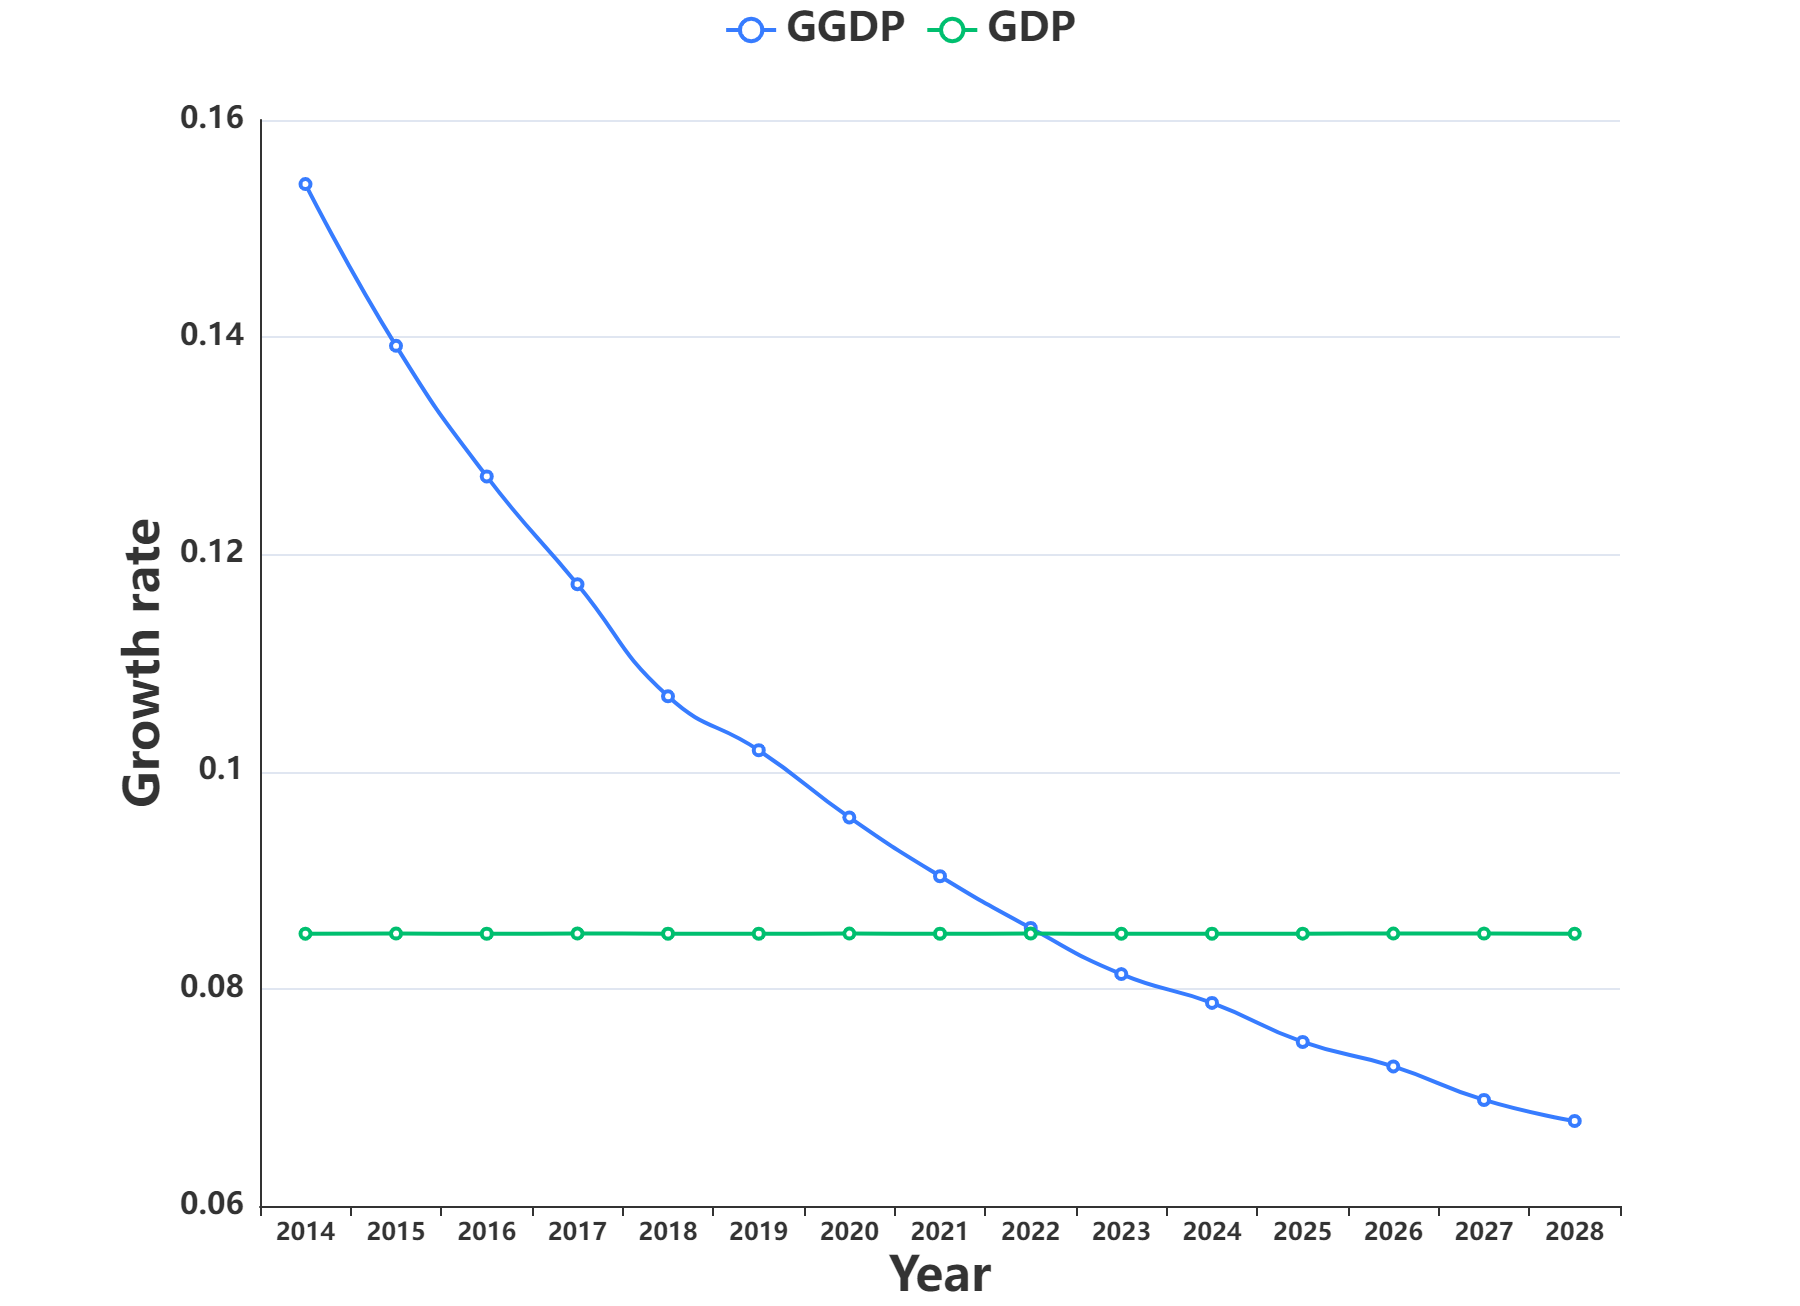
\includegraphics[width=\textwidth]{growthrate.png}
		\caption{GGDP-GDP Growth Rate}\label{fig:growthrate}
	\end{figure}

	According to the above table, the decay rate of \textit{GGDP} growth is significantly greater than \textit{GDP}.
	Because \textit{GGDP} takes the depletion of natural resources into account, this means that the depletion of natural resources is accelerating.
	To a certain extent, a country's natural resources determine the country's ability for economic development in the future.
	There is no doubt that the adoption of the \textit{GGDP} accounting system is beneficial to this country.

	
	\section{Sensitivity Analysis} %敏感性分析
	Now that we analyze the \textit{GGDP}, \textit{GDP}, \textit{GGDP}/\textit{GDP}, global carbon dioxide emissions and other data of the United States and China, in order to ensure the sensitivity of our model, we optimize and verify it in many ways.
	Considering policy-related economic factors, we use econometric models to test and optimize it, including \textbf{Autoregressive Integrated Moving Average}(ARIMA) and \textbf{Random Sample Consensus}(RANSAC). 
	
	For the \textbf{TOPSIS}, we only use the \textbf{EWM} to evaluate the indicators. Due to the limitations caused by its own principle, the \textbf{EWM} cannot consider the influence of subjective factors on the importance of indicators.
	Therefore, we use the Analytical Hierarchy Process to correct the weights subjective factors, and the final weight takes the average number of \textbf{EWM} and the Analytical Hierarchy Process.
	In this way, objective and subjective factors can be considered comprehensively, and then the model can be optimized to make it more in line with the real situation.
	
	
	\subsection{RANSAC}
	
	General regression model: 
	
	\begin{equation}\label{}
		Y_{i}=\sum_{j=1}^{p} x_{ij}\beta _{j}+e_{i}
	\end{equation}

	
	The optimized objective function is:
	
	\begin{equation}\label{}
		G_{min}=\sum_{i=1}^{n}w_{i}(Y_{i}-\sum_{j=1}^{p}x_{ij}\beta _{j} ) ^{2}
	\end{equation}
	
	Regarding the impact of \textit{GGDP} in the United States on the proportion of global renewable energy power generation, because we initially used the linear regression equation as the model, we used the \textbf{RANSAC} to test its sensitivity to obtain:
	
	\begin{equation}\label{}
		y_{energy} = 0.574x_{GGDP} -2.224	
	\end{equation}
	 
	 Through the analysis of the \textbf{RANSAC}, we can conclude that the proportion of \textit{GGDP} in the United States is positively correlated with the proportion of global renewable energy generation, and the prediction error between the prediction data and the binary linear regression equation does not exceed 8.07\%, so the model is more sensitive.
	 But when predicting the relationship between global carbon dioxide emissions and the \textit{GGDP} of the United States, we found that the model does not correctly reflect the interaction between the two variables.
	 I think the most important reason is that because changes in a single country do not necessarily affect changes in global scale, so this is also our model. Shortcomings.
	
	\begin{figure}[!htbp]
		\centering
		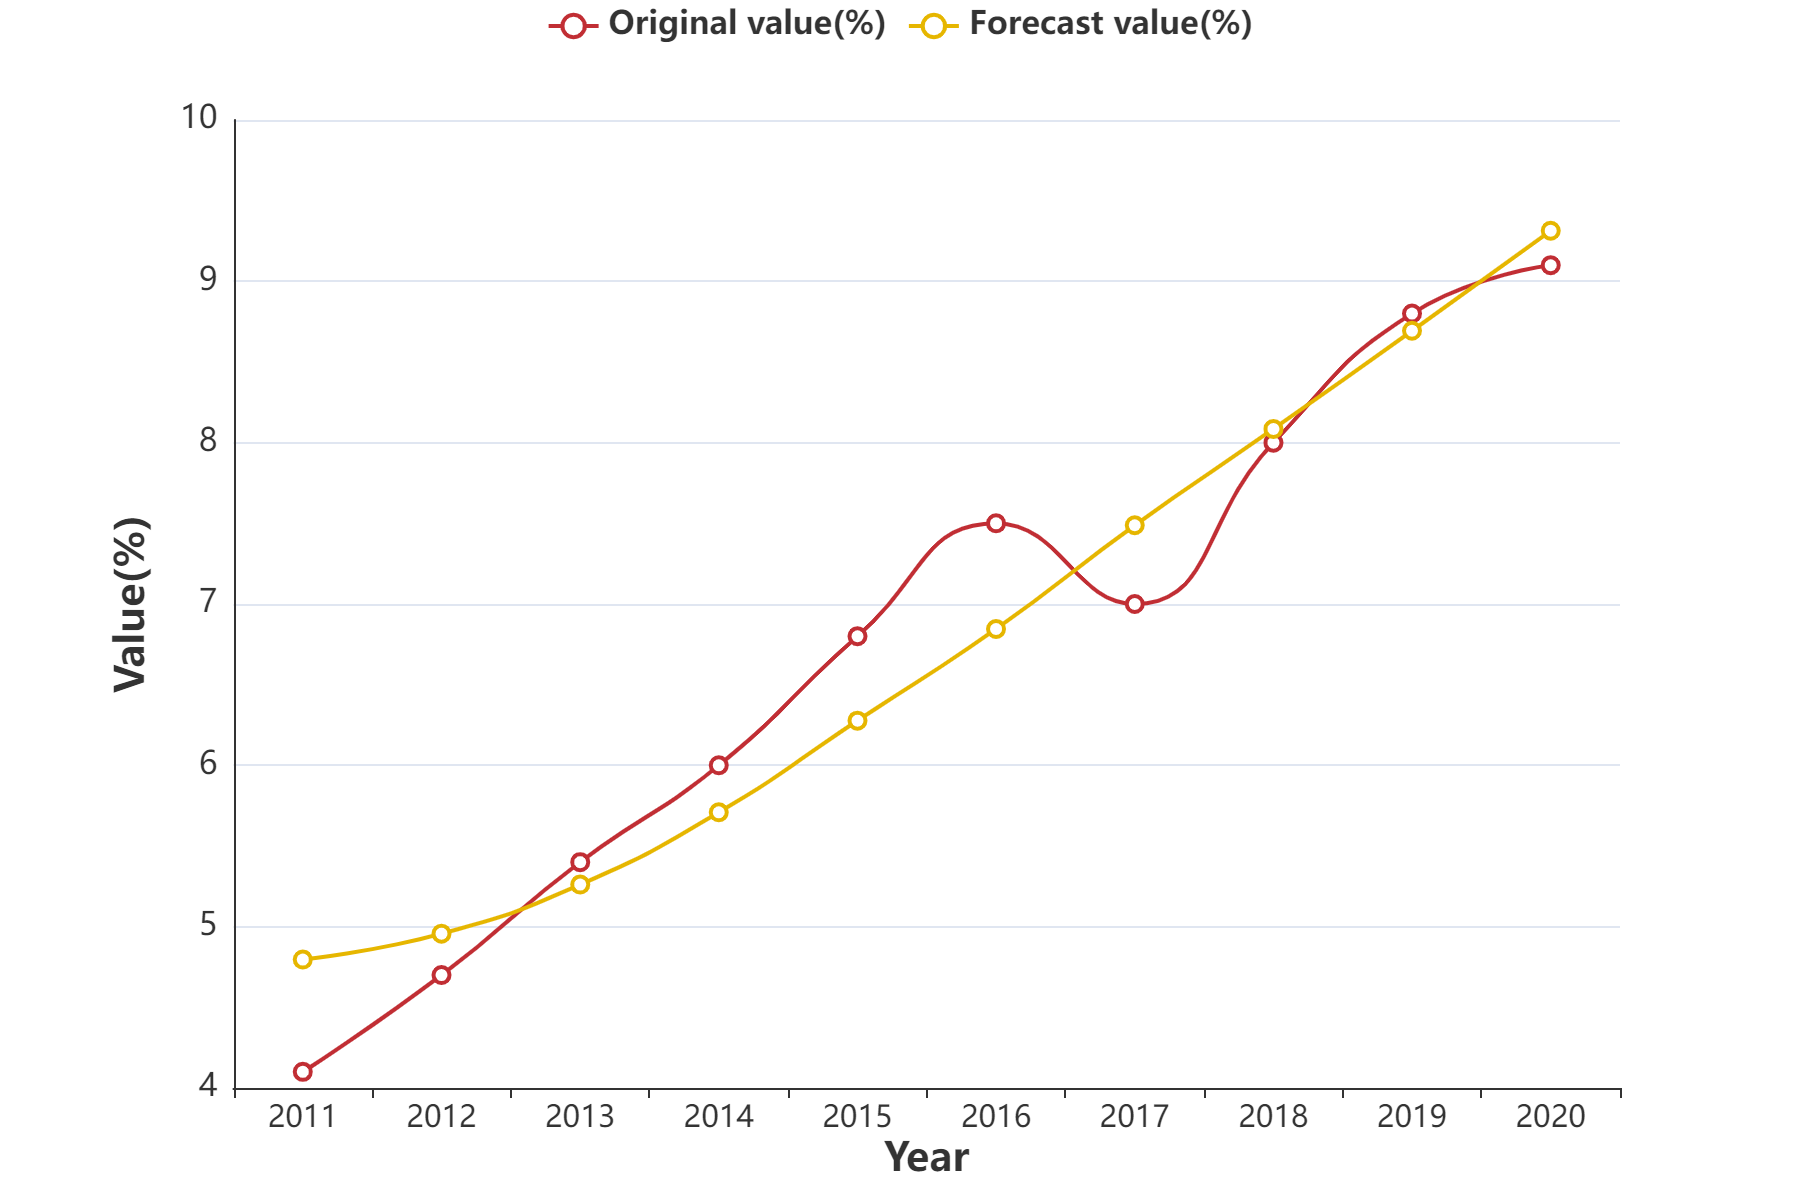
\includegraphics[width=0.8\textwidth]{RReg.png}
		\caption{RANSAC}\label{}
	\end{figure}
	
	\subsection{ARIMA}
	
	For the \textit{GGDP} trend in the United States, we use time series analysis to obtain the following difference equation: 
	\begin{equation}\label{}
		y_{t}=16.966+1.941y_{t-1}-0.996y_{t-2}
	\end{equation}

	It can be found that the trend of \textit{GGDP} predicted by the model is based on the previous model. This is consistent, so it can be concluded that the sensitivity of the model is high.
	
	\begin{equation}\label{eq:cha fen}
		\bigtriangledown^{2}y_{t}=\bigtriangledown(y_{t}-y_{t-1})
	\end{equation}

	\begin{equation}\label{eq:yan chi suan zi}
		y_{t-p}=B^{p}y_{t},\forall p\ge 1
	\end{equation}

	\begin{equation}\label{eq:ARMA pq}
		\lambda (B)(\bigtriangledown ^{d}y_{t})=\theta (B)\varepsilon _{t}
	\end{equation}
	
	\subsection{Analytical Hierarchy Process}\label{AHP}
	\textbf{AHP}, first proposed by Thomas L. Saaty, is a method used to determine weights in multi-factor hierarchical processing.
	It is widely used in safety science, environmental science and other research fields\cite{9}.
	
	\subsubsection{Build a hierarchy model}
	Through background knowledge research, the subordination model of each indicator is determined, and the indicator elements are divided into the target layer, the standard layer and the indicator layer, as shown in the figure below.
	
	\begin{figure}[!htbp]
		\centering
		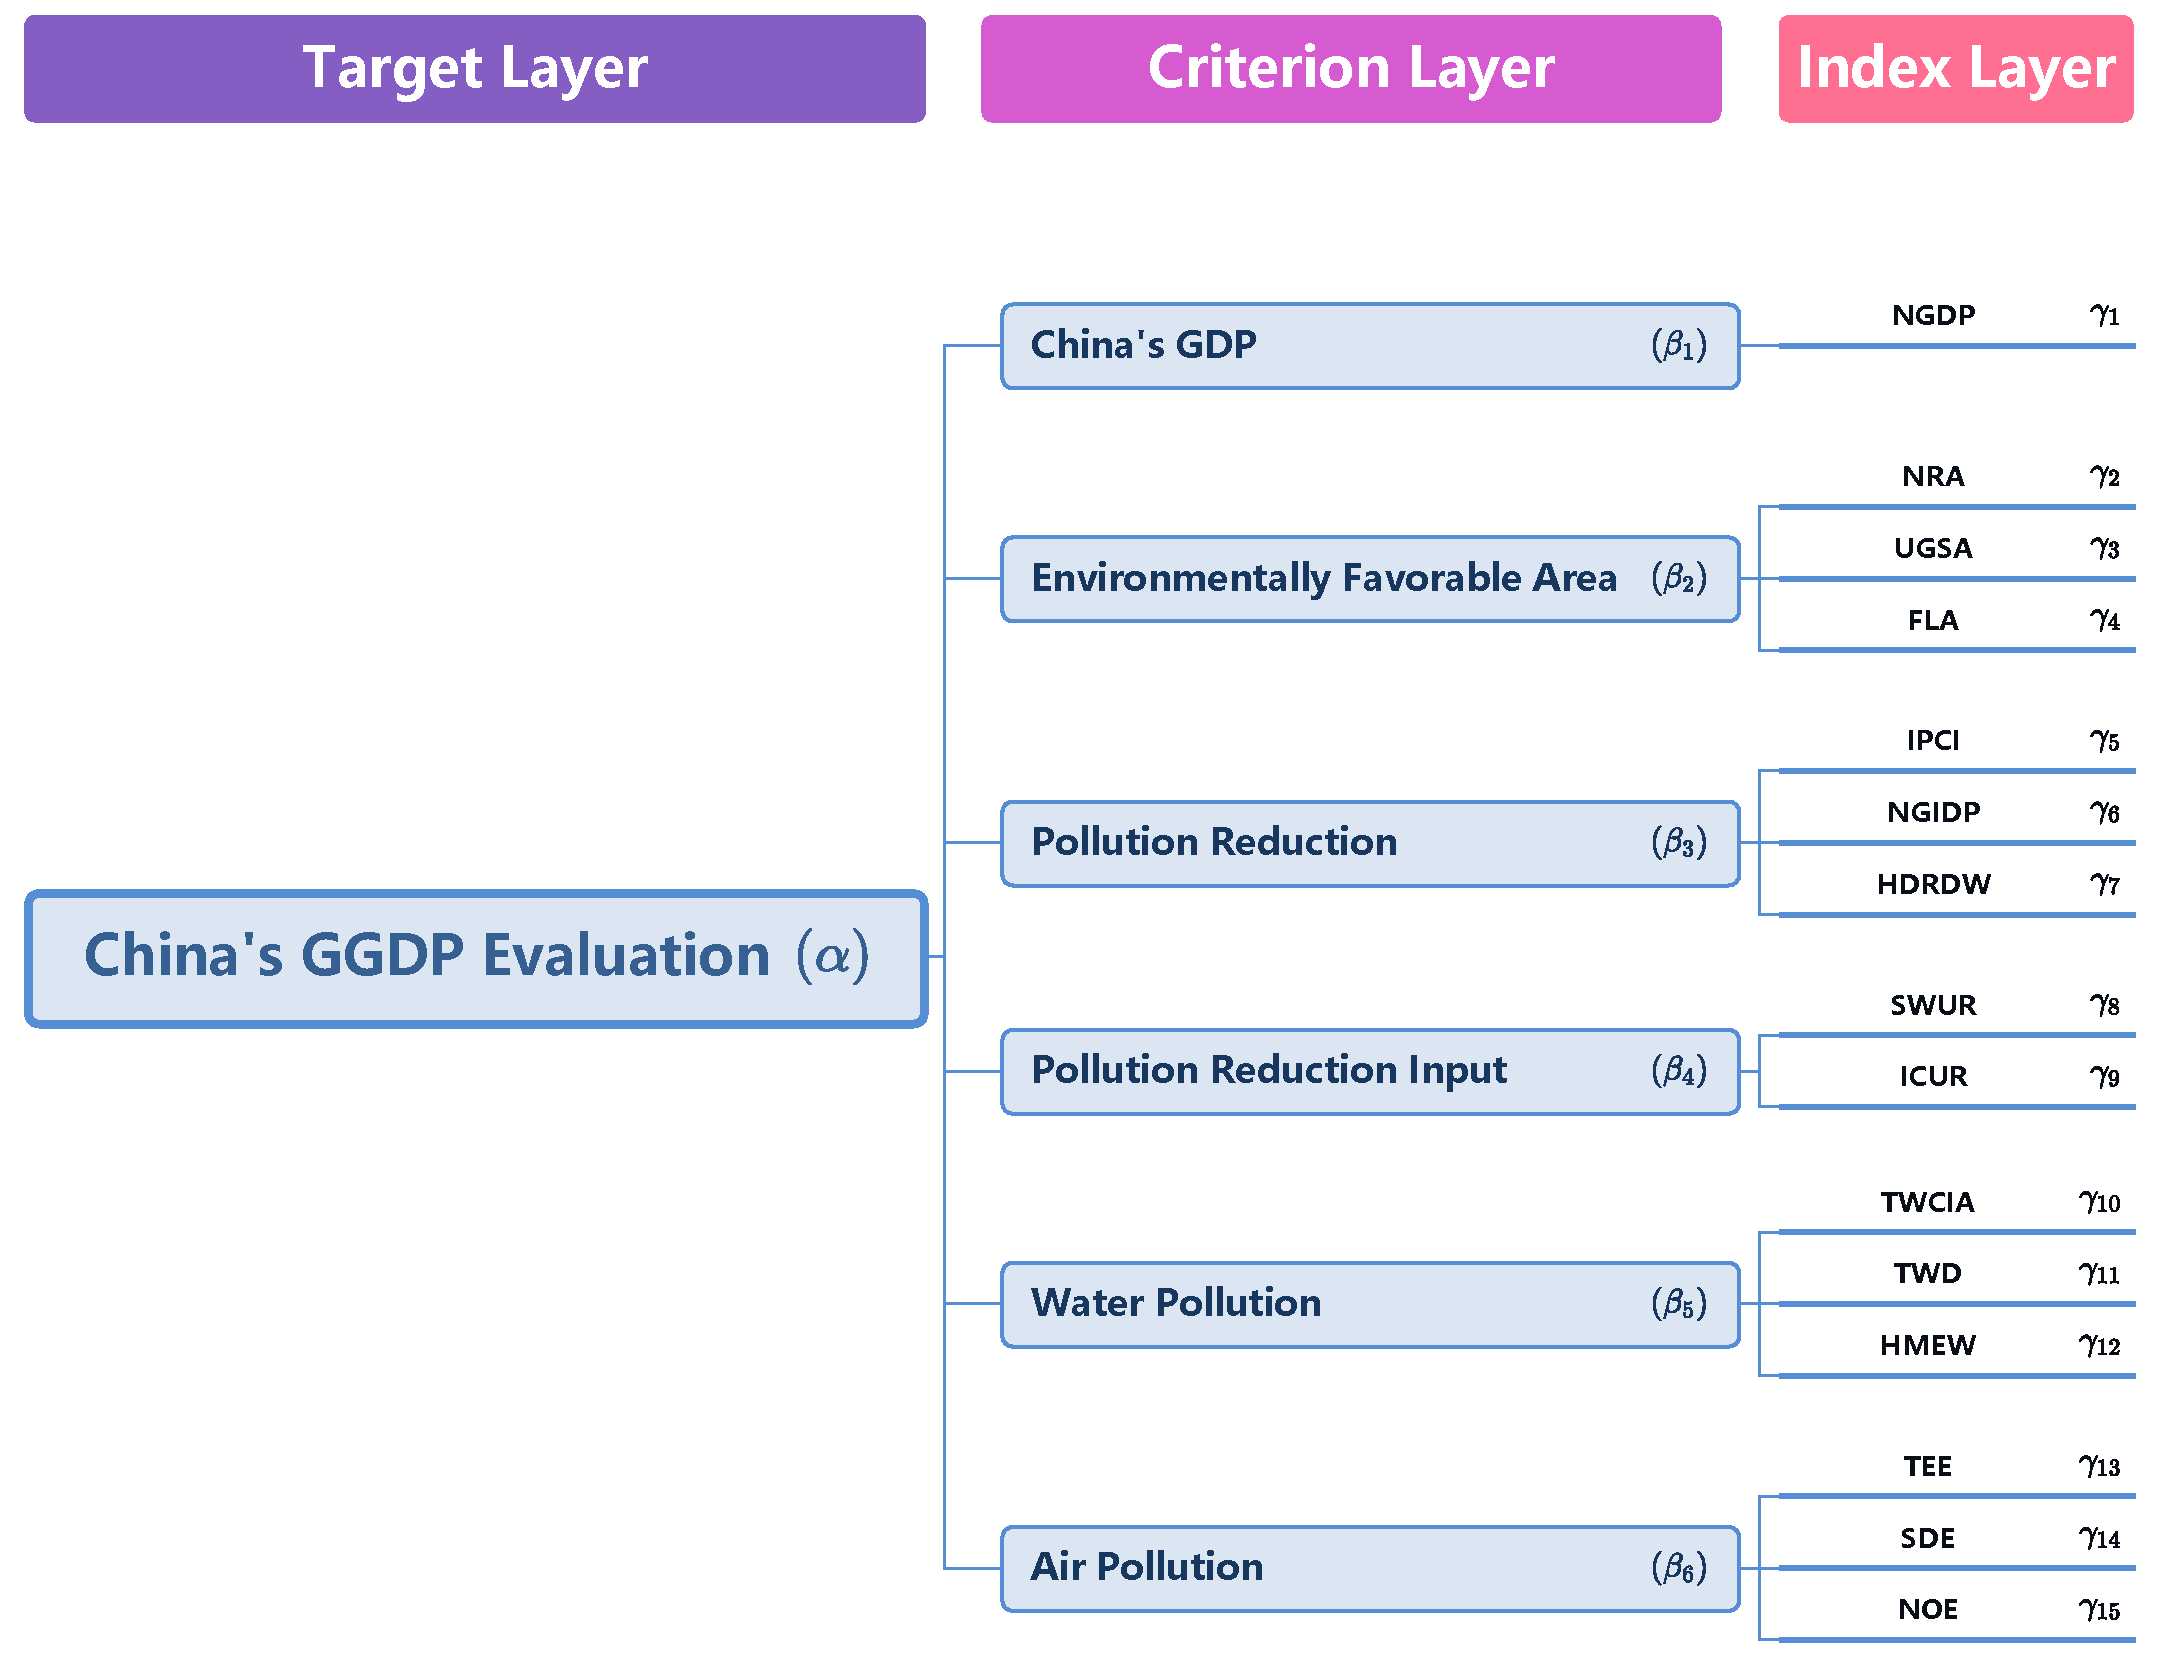
\includegraphics[width=0.8\textwidth]{China's GGDP Evaluation.pdf}
		\caption{China's GGDP Evaluation}\label{}
	\end{figure}

	\subsubsection{Construct the decision matrix}
	By judging the subjective importance of each index, the matrix is introduced to judge the scale (1-9 Scale Method)
	
	\begin{table}[!htbp]
		\begin{center}
			\caption{$1\sim9$ Scale Method}
			\label{tb:biao}
			\begin{tabular}{cc}
				\toprule
				\multicolumn{1}{m{5cm}}{\centering \textbf{Importance Scales}}
				& \multicolumn{1}{m{10cm}}{\centering \textbf{Meanings}}\\
				\midrule
				1 & the two elements are equally important \\
				3 & the former is slightly more important than the latter\\
				5 & the former is significantly more important than the latter\\
				7 & the former is more important than the latter\\
				9 & the former is extremely important than the latter\\
				2,4,6,8 & the median value of the above judgment\\
				\bottomrule
			\end{tabular}
		\end{center}
	\end{table}

	According to the hierarchical structure model, a decision matrix is established, and the criterion layer and indicator layer are calculated hierarchically.
	
	\subsubsection{Consistency test}
	In order to ensure the accuracy of the weighting indicator, the consistency test of the indicator is required.
	\begin{enumerate}
		\item Calculate the consistency index $C_{I}$, the calculation formula is:
		\begin{equation}\label{}
			C_{I} = \frac{\lambda_{max} - n}{n - 1}
		\end{equation}
		
		where
		
		\qquad $\lambda_{max}$ is the maximum eigenvalue of the judgment matrix, and $n$ is the order of the comparison matrix.
		
		\item Calculate consistency ratio $C_{R}$, calculation formula:
		\begin{equation}\label{}
			C_{R} = \frac{C_{I}}{R_{I}}
		\end{equation}
		
		where
		
		\qquad When $C_{R} < 0.1$, the judgment matrix has satisfactory consistency. $R_{I}$ represents the average random consistency index, obtained by $R_{I}$corrected value table \ref{tb:ARCI}
		\begin{table}[!htbp]
			\begin{center}
				\caption{Values of average random consistency indexes\cite{4}}
				\label{tb:ARCI}
				\begin{tabular}{ccccccccccc}
					\toprule
					\multicolumn{1}{m{1cm}}{\centering \bm{$n$}}
					& \multicolumn{1}{m{1cm}}{\centering 1}
					& \multicolumn{1}{m{1cm}}{\centering 2}
					& \multicolumn{1}{m{1cm}}{\centering 3}
					& \multicolumn{1}{m{1cm}}{\centering 4}
					& \multicolumn{1}{m{1cm}}{\centering 5}
					& \multicolumn{1}{m{1cm}}{\centering 6}
					& \multicolumn{1}{m{1cm}}{\centering 7}
					& \multicolumn{1}{m{1cm}}{\centering 8}
					& \multicolumn{1}{m{1cm}}{\centering 9}
					& \multicolumn{1}{m{1cm}}{\centering $\cdots\cdots$}\\	
					\bm{$R_{I}$} & 0 & 0 & 0.58 & 0.90 & 1.12 & 1.24 & 1.32 & 1.41 & 1.45 & $\cdots\cdots$\\
					\bottomrule
				\end{tabular}
			\end{center}
		\end{table}
	\end{enumerate}
	

	
	\subsubsection{Result}
	After testing, all decision matrices have passed the consistency test, so the weight obtained is reasonable. In order to balance objective and subjective factors, we will take the weighted average of the \textbf{EWM} \eqref{getweight} and \textbf{AHP} \eqref{AHP}, and then obtain the optimized evaluation index weight system(Table \ref{tb:system}).
	
	\begin{equation}\label{}
		W = k_{1}W_{EWM} + k_{2}W_{AHP}
	\end{equation}
	
	there
	
	\qquad $k_{1}=k_{2}=0.5$
	
	\begin{table}[!htbp]
		\begin{center}
			\caption{ Weighting system of China's GGDP evaluation index}
			\label{tb:system}
			\begin{tabular}{ccccc}
				\toprule
				\multicolumn{1}{m{3cm}}{\centering \small \textbf{Target Layer}}
				& \multicolumn{1}{m{3cm}}{\centering \small \textbf{Criterion Layer}}
				& \multicolumn{1}{m{3cm}}{\centering \small \textbf{Weight}(\%)}
				& \multicolumn{1}{m{3cm}}{\centering \small \textbf{Index Layer}}
				& \multicolumn{1}{m{3cm}}{\centering \small \textbf{Weight}(\%)}\\
				\midrule
				\multirow{15}{2cm}{\centering \small China's GGDP Evaluation} & \multirow{1}{3cm}{\centering \small China's GDP} & 26.95 & \small NGDP & 26.9500 \\ \cline{2-5}
				& \multirow{3}{3cm}{\centering \small Environmentally Favorable Area} & \multirow{3}{*}{17.6735} & \small NRA & 5.4430 \\
				&                                                 &                   & \small UGSA  & 4.8875 \\
				&                                                 &                   & \small FLA   & 7.3430 \\ \cline{2-5} 
				& \multirow{3}{3cm}{\centering \small Pollution Reduction}            & \multirow{3}{*}{11.0220} & \small IPCI  & 5.0440 \\
				&                                                 &                   & \small NGIDP & 3.7810 \\
				&                                                 &                   & \small HDRDW & 2.1970 \\ \cline{2-5} 
				& \multirow{2}{3cm}{\centering \small Pollution Reduction Input}      & \multirow{2}{*}{11.9795} & \small SWUR  & 5.8415 \\
				&                                                 &                   & \small ICUR & 6.1380 \\ \cline{2-5} 
				& \multirow{3}{3cm}{\centering \small Water Pollution}                & \multirow{3}{*}{14.5785} & \small TWCIA & 7.3075 \\
				&                                                 &                   & \small TWD & 4.2110\\
				&                                                 &                   & \small HMEW & 3.0600\\ \cline{2-5} 
				& \multirow{3}{3cm}{\centering \small Air Pollution}                  & \multirow{3}{*}{17.7965} & \small TEE  & 8.6485 \\
				&                                                 &                   & \small SDE & 5.184 \\
				&                                                 &                   & \small NOE & 3.964\\ 
				\bottomrule
			\end{tabular}
		\end{center}
	\end{table}
	
	
	\begin{figure}[htbp]
		\begin{subfigure}[b]{0.5\textwidth}
			\centering
			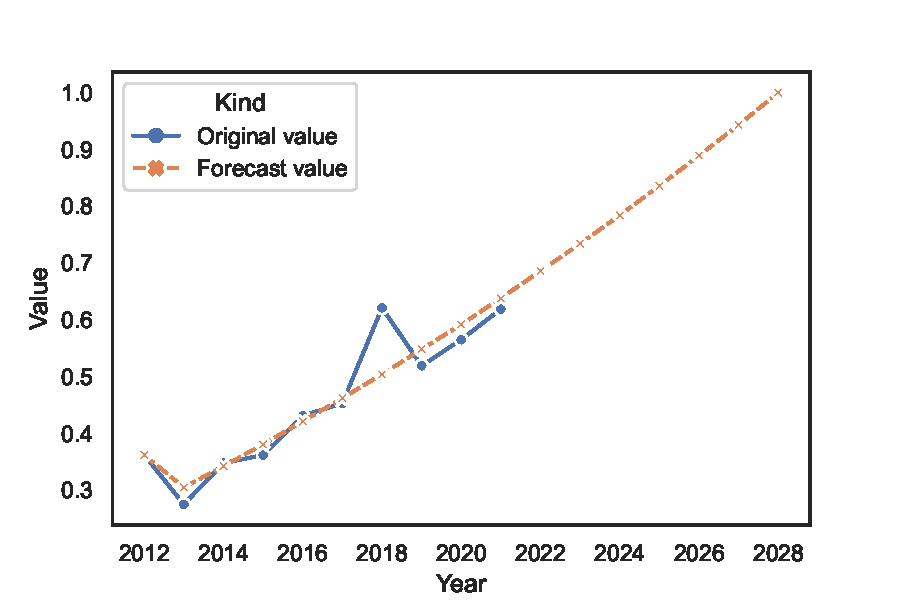
\includegraphics[width=\textwidth]{GrayModel/EWM.pdf}
			\caption{Before optimization}\label{fig:BO}
		\end{subfigure}
		\begin{subfigure}[b]{0.5\textwidth}
			\centering
			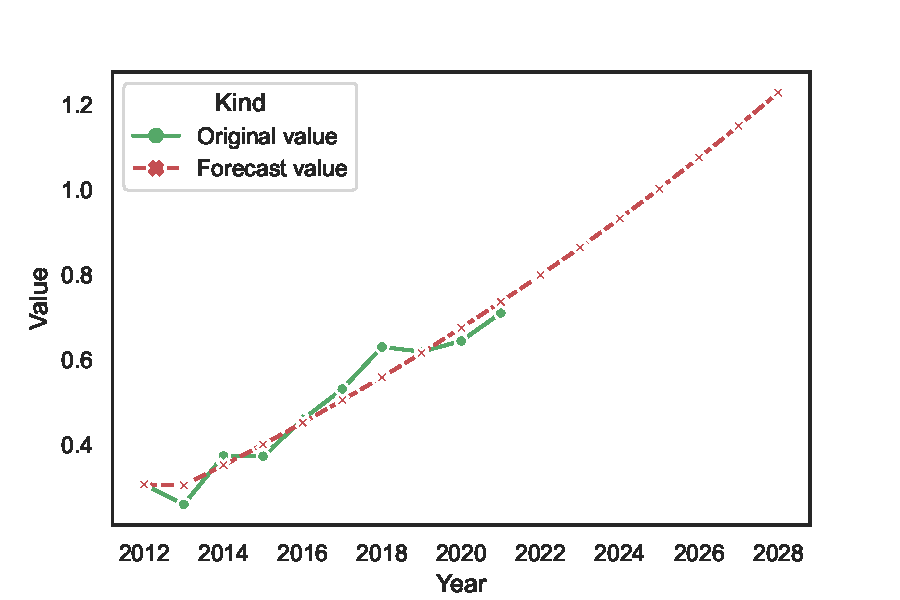
\includegraphics[width=\textwidth]{GrayModel/AHP+EWM.pdf}
			\caption{After optimization}\label{fig:AO}
		\end{subfigure}
		\caption{GM(1,1) Renderings}\label{}
	\end{figure}
	
	
	\newpage
	
	\section{Strengths and Weaknesses} %优势和劣势
	\subsection*{Strengths} %优势
	\begin{itemize}
		\item Most of the mathematical models we create are highly sensitive and adopt the comprehensive considerations of econometric models, mathematical prediction models and mathematical evaluation models, so they can reflect the actual impact of changes more objectively and realistically.
		\item We use a variety of weight analysis methods to obtain more comprehensive weights, and then modify the original weight to make our prediction model more accurate.
		\item Based on our reasonable assumptions, we put forward policy suggestions to our leaders that are more conducive to the healthy development of the country's economy.
	\end{itemize}
	
	\subsection*{Weaknesses} %劣势
	\begin{itemize}
		\item Due to the diversification of government values in various countries, our model may not be able to predict future accuracy more accurately in every country.
		\item Because the proportion of a single country's global impact is relatively small, the prediction model of the global impact of a single country may be biased.
	\end{itemize}
	
	\newpage
	
	% 参考文献,此处以 MLA 引用格式为例
\begin{thebibliography}{99}
		\bibitem{1} Scientific Platform Serving for Statistics Professional 2021. SPSSPRO. (Version 1.0.11)[Online Application Software]. Retrieved from\url{https://www.spsspro.com}
		\bibitem{2} \emph{A simple, easy \LaTeX\ template for MCM/ICM: EasyMCM}. (2018). Retrieved December 1, 2019, from\url{https://www.cnblogs.com/xjtu-blacksmith/p/easymcm.html}
		\bibitem{3} U.S. Energy Information Administration. Retrieved from \url{https://www.eia.gov}
		\bibitem{4} World Bank Open Data. Retrieved from \url{https://data.worldbank.org}
		\bibitem{5} The State Council,The People's Republic of China. Retrieved from \url{https://www.gov.cn}
		\bibitem{6} National Bureau of Statistics of China. Retrieved from \url{http://www.stats.gov.cn}
		\bibitem{7} Ministry of Ecology and Environment of the People's Republic of China. Retrieved from \url{https://www.mee.gov.cn}
		\bibitem{8} Shih H S, Shyur H J, Lee E S. An extension of TOPSIS for group decision making[J]. Mathematical \& Computer Modelling, 2007, 45(7):801-813.
		\bibitem{9} Liu Zhao." Visual landscape quality evaluation of Taiyuan Suburban Forest Park based on AHP method. Journal of Zhongnan University of Forestry Science and Technology .02(2023):188-200. doi:10.14067/j.cnki.1673-923x.2023.02.020.
		\bibitem{10} Liu Shouying. Continue to be obsessed with high growth or prevent contraction.Retrieved from \url{https://m.thepaper.cn/baijiahao_8666511}
		
\end{thebibliography}
	
	
\end{document}
